\documentclass[11pt]{article}

% Figures
\usepackage{graphicx}
\usepackage[list=true]{subcaption}
\graphicspath{{../../plots/}{../../tikz/}{../../img/}}
\usepackage[section]{placeins} % require floats to appear in the section they are defined

% fonts and appearance
\usepackage{amsmath, amsfonts, physics, siunitx, nicefrac}
\usepackage[american]{babel} 
\usepackage[T1]{fontenc} % improved font encoding
\usepackage[ttscale=0.8]{libertine}
\usepackage{fontawesome5}
\usepackage[format=plain, textfont=it]{caption}

% page size and margins
\usepackage{geometry}
\geometry{letterpaper,top=1in, bottom=1in, left=1in, right=2in}

% footer
\usepackage{fancyhdr}
\usepackage{lastpage}
\usepackage[en-US]{datetime2}
\fancyhf{}
\fancyhead[L]{CONFIDENTIAL DRAFT by J. Doss-Gollin \& K. Keller}
\fancyhead[R]{\DTMnow}
\fancyfoot[R]{page~\thepage~of~\pageref{LastPage}}
\pagestyle{fancy}

% TO DO NOTES
\usepackage{xcolor} % list of colors at https://en.wikibooks.org/wiki/LaTeX/Colors
\definecolor{giallo}{HTML}{F0BC42} % https://teamcolorcodes.com/a-s-roma-color-codes/
\definecolor{rosso}{HTML}{8E1F2F}
\definecolor{grigio}{HTML}{CACACC}
\definecolor{nero}{HTML}{000000}
\usepackage[textsize=scriptsize]{todonotes}
\setlength{\marginparwidth}{1.5in}
\newcommand{\james}[1]{\todo[color=giallo, textcolor=nero]{\textbf{ATTN James:~}#1}} % if desired create a custom command for each author
\newcommand{\klaus}[1]{\todo[color=rosso, textcolor=grigio]{\textbf{ATTN Klaus:~}#1}}

% better tables
\usepackage{booktabs}
\usepackage{array}
\newcommand{\PreserveBackslash}[1]{\let\temp=\\#1\let\\=\temp}
\newcolumntype{C}[1]{>{\PreserveBackslash\centering}p{#1}}
\newcolumntype{R}[1]{>{\PreserveBackslash\raggedleft}p{#1}}
\newcolumntype{L}[1]{>{\PreserveBackslash\raggedright}p{#1}}

% better lists
\usepackage[inline]{enumitem}
\setlist{nosep}

% authors
\usepackage{authblk}
\title{A subjective Bayesian framework for synthesizing deep uncertainties in climate risk management}
\author[1]{James Doss-Gollin}
\author[2]{Klaus Keller}
\affil[1]{Department of Civil and Environmental Engineering, Rice University}
\affil[2]{Thayer School of Engineering, Dartmouth College}
\renewcommand*{\Affilfont}{\normalsize\normalfont}

% ACRONYMS
\usepackage[acronym,nopostdot,nonumberlist,shortcuts,]{glossaries}
\newacronym{abc}{ABC}{approximate Bayesian computation}
\newacronym{bdt}{BDT}{Bayesian decision theory}
\newacronym{bfe}{BFE}{base flood elevation}
\newacronym[]{cdf}{CDF}{cumulative distribution function}
\newacronym{fema}{FEMA}{the Federal Emergency Management Agency}
\newacronym{gcm}{GCM}{general circulation model}
\newacronym[]{gev}{GEV}{generalized extreme value}
\newacronym{iid}{IID}{independent and identically distributed}
\newacronym{ipcc}{IPCC}{International Panel on Climate Change}
\newacronym{mcmc}{MCMC}{Markov Chain Monte Carlo}
\newacronym{msl}{MSL}{mean relative sea level}
\newacronym{noaa}{NOAA}{the National Oceanic and Atmospheric Administration}
\newacronym{pdf}{PDF}{probability density function}
\newacronym{rcp}{RCP}{representative concentration pathway}
\newacronym{rdm}{RDM}{robust decision making}
\newacronym{slr}{SLR}{sea level rise}
\newacronym{ssp}{SSP}{shared socio-economic pathway}
\newacronym[plural=SOWs,descriptionplural=states of the world]{sow}{SOW}{state of the world}
\newacronym{tc}{TC}{tropical cyclone}

\usepackage{xspace}
\makeatletter
\DeclareRobustCommand\onedot{\futurelet\@let@token\@onedot}
\def\@onedot{\ifx\@let@token.\else.\null\fi\xspace}
\def\eg{\emph{e.g}\onedot} \def\Eg{\emph{E.g}\onedot}
\def\ie{\emph{i.e}\onedot} \def\Ie{\emph{I.e}\onedot}
\def\etc{\emph{etc}\onedot} \def\vs{\emph{vs}\onedot}

\usepackage{xspace}
\makeatletter
\DeclareRobustCommand\onedot{\futurelet\@let@token\@onedot}
\def\@onedot{\ifx\@let@token.\else.\null\fi\xspace}
\newcommand{\usd}[1]{\SI{#1}[\$]{}}
\def\eg{\emph{e.g}\onedot} \def\Eg{\emph{E.g}\onedot}
\def\ie{\emph{i.e}\onedot} \def\Ie{\emph{I.e}\onedot}
\def\etc{\emph{etc}\onedot} \def\vs{\emph{vs}\onedot}

% use biblatex
\usepackage{csquotes}
\usepackage[
  backend=biber,
  doi=true,
  url=false,
  isbn=false,
  style=authoryear-comp,
  natbib=true,
  backref=false,
  maxbibnames=10,
  maxcitenames=2,
  uniquename=false,
  uniquelist=false,
  sorting=nyt,
  giveninits=true,
]{biblatex}
\renewbibmacro{in:}{}
\AtEveryBibitem{\clearfield{month}\clearfield{day}\clearfield{pages}\clearlist{language}}
\addbibresource{library.bib}

% load this last
\usepackage[hidelinks]{hyperref}
\usepackage{cleveref}

% up to 1250 words
\begin{document}
\maketitle
\thispagestyle{empty}

\begin{abstract}
    National agencies, regional governments, and individual households manage flood risk through a combination of standards and cost-benefit analyses that rely on estimates of flood hazard.
    One example is house elevation: \acrlong{fema} recommends a house located in the floodplain be elevated to the \acrlong{bfe} (typically the 100 year flood level) plus a freeboard (typically \SI{1}{ft}) if doing so would pass a cost-benefit test.
    Under stationarity, the probabilities used for this analysis (\ie to estimate the 100 year flood height or to perform the cost-benefit analysis) can be estimated using empirical frequencies from the observational record.
    However, growing recognition of nonstationarity motivates a forward-looking approach.
    Efforts to incorporate nonstationarity hazard into planning have struggled to overcome deep uncertainties in projections of future hazard because different models  may fit the observed data equally well but yield very different estimates of future hazard, and there is often no objective way to choose between them (\ie, equifinality).
    In this paper we use a didactic case study of deciding if and how high to elevate a single house in the coastal zone to illustrate a decision theoretic framework that combines exploratory modeling, robust decision making, and subjective Bayesian philosophy.
    We first use exploratory modeling to illustrate that there is no dominant strategy; instead, there are instrinsic tradeoffs between performance under low- and high-\gls{slr} scenarios.
    Next, we map the tradeoff between up-front cost and expected damages for each of sixteen models of future \gls{slr} to illustrate that the choice of which model to use has a strong influence on estimated trade-offs, cost-benefit analyses, or policy prescriptions.
    To overcome these shortcomings, we propose and illustrate a computationally efficient method for scenario weighting conditional on a subjective prior belief over future \gls{slr}.
    This method provides a transparent framework for synthesizing deep uncertainties, facilitating critique and dialogue around necessarily subjective decisions.
    It can be applied beyond nontationary flood risk management to other problems in climate adaptation, calculating the social cost of carbon, and more.
\end{abstract}

Key points
\begin{enumerate}
    \item
\end{enumerate}

\clearpage
\section{Introduction}\label{sec:introduction}

Flood risk management relies on probabilistic estimates of flood hazard:
\begin{enumerate}
    \item In many countries including the United States, flood risk management involves many different public and private sector actors but most rely on probabilistic estimates of flood hazard.
    \item Local governments can build infrastructure to reduce flood risk; they often prioritize these by considering a reduction in damages from a design storm (\eg, the 100 year storm) \citep{hcfcd_prioritization:2019}
    \item There is a role for industry organizations that set standards that local governments often incorporate into building codes \citep{asce_infrastructure_climate:2021}
    \item The National Flood Insurance Program was designed as a partnership between the federal government and local communities; communities can voluntarily join the program by adopting a floodplain ordinance based on the most up-to-date flood hazard maps provided by FEMA. At a minimum, communities that choose to join must require that new development and substantially improved or damaged properties in high hazard areas be built at or above the level of a flood with a return period of one in 100 years (i.e., the 100-year flood). \citep{kousky_voucher:2014}
    \item Beyond flood insurance and disaster recovery there has been a federal retreat from flood risk management leaving local governments and individuals with most of the responsibility for flood risk management: ``the federal government recognizes its risks as a major owner and operator of infrastructure, facilities, \ldots, and insurer of properties and crops \ldots leaving states, localities, and individual agencies to make their own plans'' \citep{shi_transformative:2021}
\end{enumerate}
Future flood hazard is deeply uncertain
\begin{enumerate}
    \item ``Along the U.S. coastline, public infrastructure and \$1 trillion in national wealth held in coastal real estate are threatened by rising sea levels, higher storm surges, and the ongoing increase in high tide flooding'' \citep{reidmiller_reportinbrief:2018}
    \item Nonstationarity also affects inland and pluvial flooding \citep{Milly:2008dg} and derives from a combination of climate change, land use change, and local river modifications \citep{Merz:2014gf}
    \item Federal guidelines for flood risk management that directly inform policy-making recognize the presence of nonstationarity but have failed to identify objectively valid approaches for modeling nonstationarity, \citep{Montanari:2014hl,Serinaldi:2015bq}
    \item For coastal flooding, \gls{fema} guidance suggests using up to date estimates of \gls{msl} \citep{fema_slr:2016}, but no projections, and stationary estimates of storm surge \citep{fema_ffa:2016}, although the analyst at each location has considerable flexibility
    \item Ditto extreme rainfall \citep{atlas14_texas:2018} or floods \citep{bulletin17c:2019}
    \item This is because where historic flood risk can be constrained by estimates, future flood risk depends on intrinsically unpredictable human decisions like greenhouse gas emissions, and is therefore deeply uncertain \citep{keller_management:2021}
\end{enumerate}
Methods for decision making under deep uncertainty emphasize exploring many possible futures
\begin{enumerate}
    \item deep uncertainty describes ``known unknowns'' where there is not a single objectively true model \citep{walker_deep:2013,Walker:2013gi,lempert_complex:2002}
    \item This is related to equifinality where different models fit the historical record equally well but diverge as one looks into the future \citep{beven_equifinality:2006,DossGollin:2019}
    \item Applying classical optimization methods to problems with deep uncertainty can yield highly fragile solutions in the sense that
    \item \citet{bankes:1993} draws a distinction between exploratory and consolidative modeling
    \item Decision scaling \citep{Steinschneider:2015kk}
    \item global sensitivity analysis \citep{saltelli_sensitivity:2010,herman_salib:2017,sobol_sensitivity:2001} use feed large scenario ensembles into a black box model, then analyze outputs to assess the relative importance of each input (conditional on an assumed joint distribution over inputs)
    \item MORDM \citep{kasprzyk:2013} combines exploratory modeling (exploring performance over many scenarios) and policy search (using optimization tools)  \citep{kasprzyk:2013,kasprzyk_denovo:2012,hadka_mordm:2015}. Typically ``robustness metric'' is used \citep{herman:2015,mcphail_robustness:2019}
    \item For a more complete review see \citet{marchau:2019}
    \item RDM-like methods have been applied to coastal infrastructure planning by sampling \glspl{sow} from a \gls{pdf} of \gls{slr}, then identifying decisions that meet some predetermined satisficing criteria \citep{mcphail_robustness:2019} over a large fraction of possible futures \citep{sriver_sealevel:2018,garner_slrise:2018,lempert_slr:2012}
    \item Crucially, these approaches all emphasize exploring performance over many scenarios, then describing this performance into some set of metrics.
\end{enumerate}
Some critiques
\begin{enumerate}
    \item There are always subjective  modeling decisions, but sometimes they are opaque which makes it hard to communicate them to the end user
    \item The range you choose is also subjective! \citep{schneider_dangerous:2001,schneider_scenarios:2002}
    \item Technical detail: joint probability distributions over high dimensional spaces are confusing. Bayesian analysis teaches us that posterior distributions of parameters are often highly correlated. If we neglect that by sampling over the marginal distribution of each parameter separately, we may be sampling almost entirely from regions of the parameter space that are not consistent with our data!
    \item Some scenarios are more likely than others \citep{hausfather_scenarios:2020,ho_scenarios:2019} yet this is generally not acknowledged
\end{enumerate}
The question of whether probability is a useful tool for decision making under deep uncertainty depends on how one interprets probability; we argue that a subjective Bayesian interpretation of probability is useful for many DMDU problems
\begin{enumerate}
    \item We are inspired by methods and philosophy of Bayesian model choice in the ``$\mathcal{M}$-open'' case where there is no true model to identify
    \item Many modern discussions of Bayesian philosophy \citep{jaynes_probability:2003,McElreath:2016vu,Gelman:2014tc,bernardo_bayesian:1994} also emphasize a philosophical view of probability as a language with which to reason about the unknown rather than a statement of objective truth \citep[see][for a thorough discussion of Bayesian philosophy]{gelman_philosophy:2013}. This is in many ways closer to the exploratory modeling proposed by \citet{bankes:1993} than the top-down, deterministic, fragile central planning approaches that it (and \cite{rittel:1973} and others) critiqued
    \item \gls{bdt} was conceived as a calculus for reasoning rather than for identifying objective truth; \citeauthor{definetti_probability:1972} often said that ``probability does not exist'' \citeyear{definetti_probability:1972}. \citet{savage:1954} and \citet{ramsey_probability:2016}, among others, also viewed probability as ``subjective,'' representing the state of belief of the decision-maker.
    \item We know that choosing a single ``best'' model under-estimates uncertainty so inferences need to be combined across models \citep[\eg, as in stacking;][]{Yao:2018bu}
    \item In the absence of data that would tell us how accurate each model is via some likelihood function, we have to use the prior.
    \item The famous phrase ``all models are wrong, but some are useful'' \citep[generally attributed to][]{box:1976} also suggests that probability distributions and predictions ought to be viewed subjectively.
    \item Although the true data generating process is not known and inference should not be represented as objective truth, probability gives a transparent and consistent language for reasoning about uncertainty.
    \item Since modeling assumptions cannot overcome epistemic uncertainty, even with better models and more data, we draw from the literature on statistical model selection in the $\mathcal{M}$-open setting, which provides a theoretical background for choosing between models when the true data generating process is not among the models considered \citep[see][]{Piironen:2017eh}.
    \item Often, combining inferences from multiple models is more effective than seeking a single ``best'' model \citep{Yao:2018bu}. More fundamentally, this literature emphasizes the importance of iteratively building models, simulating the consequences of those models, and critiquing them \citep{gelman_workflow:2020}.
    \item Since, by definition, models are not ``true,'' this iterative workflow \citep{gelman_workflow:2020} aims to identify models that are useful and promote a dialog amongst stakeholders \citep{gelman_philosophy:2013}
\end{enumerate}
Our aim is to illustrate how methods for model selection in the $\mathcal{M}$-open case can improve decision making under deep uncertainty.
\begin{enumerate}
    \item We want to combine multiple models in a way that is transparent, and that can be changed with low computational cost (cheap robustness checks).
    \item We are particularly motivated by problems for which simulations of some key uncertainties (particularly climate-driven ones but also population, economic growth, etc) already exist. We assume only that there is no coupling between the system model and these simulations, so they can be treated as fully exogenous.
\end{enumerate}
We illustrate our approach with a didactic case study\ldots.
\begin{enumerate}
    \item House elevation in the coastal zone as a specific example of a problem where both over- or under-investment could be a problem
    \item Federal guidance uses both standards (floodplain, \gls{bfe}) and cost-benefit analysis (does it pass test?)
    \item Be sure to note that this has parallels to lots of other engineering design guidance.
    \item \citet{xian_elevation:2017}: one size does not fit all
    \item \citet{zarekarizi_suboptimal:2020}: neglecting uncertainty leads to bad outcomes
    \item Prior studies have found that floodproofing and building-scale vulnerability reduction measures, including house elevation, can effectively reduce local flood damages in many contexts \citep{demoel_reducing:2014,deruig_building:2020,kreibich_building:2005,slotter_floodproofing:2020,Rozer:2016dn,mobley_mitigation:2020,aerts_cost:2018}.
    \item Official guidance for homeowners, notably from \gls{fema}, recommends elevating to the \gls{bfe} (typically the \SI{100}{year} flood) plus a freeboard \citep{fema_retrofitting:2014,asce_24-14:2015,fema_retrofitting:2014} but recent suggests scope for improvement.
    \item For example, \citet{xian_elevation:2017} uses a cost-benefit analysis to demonstrate that tailoring recommendations to the initial elevation of a structure can reduce expected costs.
          \citet{zarekarizi_suboptimal:2020} show that neglecting uncertainty in discount rate, house lifespan, flood risk, and depth-damage curves can lead to maladaptation.
    \item Yet these studies are silent on the question of how nonstationary flood hazard should factor into this decision.
    \item FEMA's Hazard Mitigation Grant Program, authorized under Section 404 of the 1988 Stafford Act, which awards grants after a disaster. Under the Stafford Act, projects funded by HMGP, including buyouts, must be shown to be cost-effective; typcally, up-front costs are compared to avoided losses \citep{bendor_buyouts:2020}
\end{enumerate}
Our primary research question is ``how can deep uncertainties be transparently and consistently synthesized for decision analysis?''
We proceed as follows.
\begin{enumerate}
    \item In \cref{sec:case-study} we describe our case study in Norfolk, VA.
    \item  in \cref{sec:exploratory} we analyze each simulation (\ie, realizations from these \glspl{pdf}) independently and illustrate .
    \item  in \cref{sec:multiple-pdf} we consider the design problem as a set of ``multiple \glspl{pdf}'' and use these findings to motivate theoretical advances.
    \item  in \cref{sec:synthesizing} we present a probabilistic method for synthesizing simulations from multiple \glspl{pdf} and illustrate the advantages and potential pitfalls of this approach.
    \item  in \cref{sec:conclusions} we briefly summarize our findings, discuss implications for engineering practice, and identify  future research needs.
\end{enumerate}


\section{Case study}\label{sec:case-study}

We model one-time decision of whether to elevate a house, and if so by how much (\cref{fig:xlrm}), for a \emph{hypothetical} house in Norfolk, VA.
For interpretability, we focus on deep uncertainty in \gls{msl} and treat other model parameters as more shallow uncertainties as shown in \cref{tab:uncertainties}.

\begin{table}
    \centering
    \caption{
        Summary of parameters, their notation, and how their uncertainty is represented.
    }\label{tab:uncertainties}
    \begin{tabular}{l l p{3in} l}
        \toprule
        Name             & Symbol            & Uncertainty                                                                          & See more                     \\
        \midrule
        \Gls{msl}        & $\overline{y}(t)$ & Deeply uncertain: four physical models $\times$ four \acrshort{rcp} scenarios        & \cref{sec:sea-level}         \\
        Storm surge      & $y'(t)$           & Probabilistic: Bayesian inference on a stationary \acrshort{gev} model               & \cref{sec:storm-surge}       \\
        Ann-max flood    & $y(t)$            & Deterministic: $y(t)=\overline{y}(t)+y'(t)$                                          &                              \\
        Discount rate    & $1-\gamma$        & Fixed at 3\%                                                                         & \cref{sec:led}               \\
        Depth-damage     & $D(h-y)$          & Deterministic: based on HAZUS model                                                  & \cref{fig:cost-depth-damage} \\
        Elevation cost   & $C(\Delta h)$     & Deterministic: a piecewise linear model following \citet{zarekarizi_suboptimal:2020} & \cref{fig:cost-up-front}     \\
        Initial height   & $h_0$             & Deterministic: \SI{1}{ft} below the \gls{bfe} unless otherwise noted                 &                              \\
        House floor area &                   & Deterministic: \SI{1500}{ft^2} unless otherwise noted                                &                              \\
        Structural value &                   & Deterministic: \usd{200000} unless otherwise noted                                   &                              \\
        House lifetime   &                   & Deterministic: 70 years unless otherwise noted                                       &                              \\
        First year       & $t_i$             & Deterministic: 2022                                                                  &                              \\
        Last year        & $t_f$             & Deterministic: 2091 unless otherwise noted                                           &                              \\
        \bottomrule
    \end{tabular}
\end{table}

\begin{figure}
    \centering
    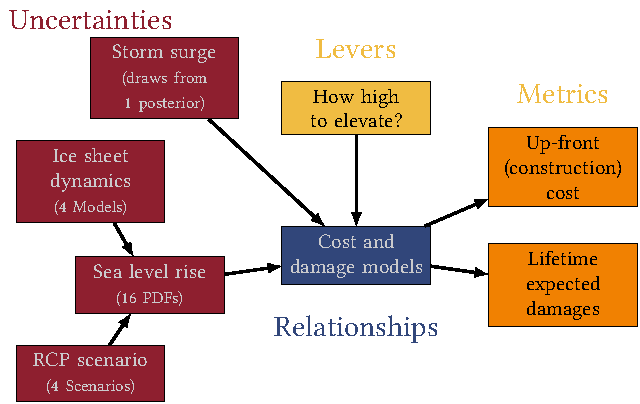
\includegraphics[width=\textwidth]{xlrm.pdf}
    \caption{
        Conceptual diagram of the decision problem.
        A \gls{sow} consists of a description of the uncertain factors (red).
        We model a problem with a single lever (yellow), which is how high to elevate a house ($\Delta h$).
        For each \acrshort{sow} and each value of $\Delta h$, the system model (blue) is used to calculate performance metrics (orange).
    }\label{fig:xlrm}
\end{figure}

\subsection{\gls{slr}}\label{sec:sea-level}

To inform the house elevation decision, we develop an ensemble \gls{msl} time series.
Specifically, we analyze simulations of \gls{msl} at Sewells Point, VA from four probabilistic physical models using data published in \citet{ruckert_coastal:2019}.
The four models considered are (i) the BRICK model (version 0.2) with slow (``BRICK Slow'') and (ii) fast (``BRICK Fast'') ice sheet dynamics \citep{wong_brick0.2:2017}, (iii) the \citet{kopp_probabilistic:2014} model (``K14''), and (iv) the \citet{deconto_antarctica:2016} model (``DP16'').
The \citet{kopp_probabilistic:2014} and \citet{deconto_antarctica:2016} models have a ten year time step, which we linearly interpolate onto a one year time step for consistency.
These four models represent physical processes, particularly of ice sheet dynamics, in different ways, leading to diverging sensitivity of \gls{msl} to forcing.
For a discussion of these methods, their similarities, their differences, and their consistency with other analyses see \citet{ruckert_coastal:2019}, \citet{kopp_evolving:2017}, and \citet{bamber_slrise:2019}.

Estimates of nonstationary \gls{msl} also depend on anthropogenic forcing, which is itself deeply uncertain.
To sample this uncertainty, we use simulations from each physical model under four \gls{rcp} scenarios, yielding sixteen time-varying probability density functions of \gls{msl}.
We refer to each time series of \gls{msl}, $\overline{y}(t)$, as \emph{a \acrfull{sow}} and to each combination of physical model and \gls{rcp} scenario as \emph{a model} for $p(\overline{y}|t)$.

\begin{figure}
    \centering
    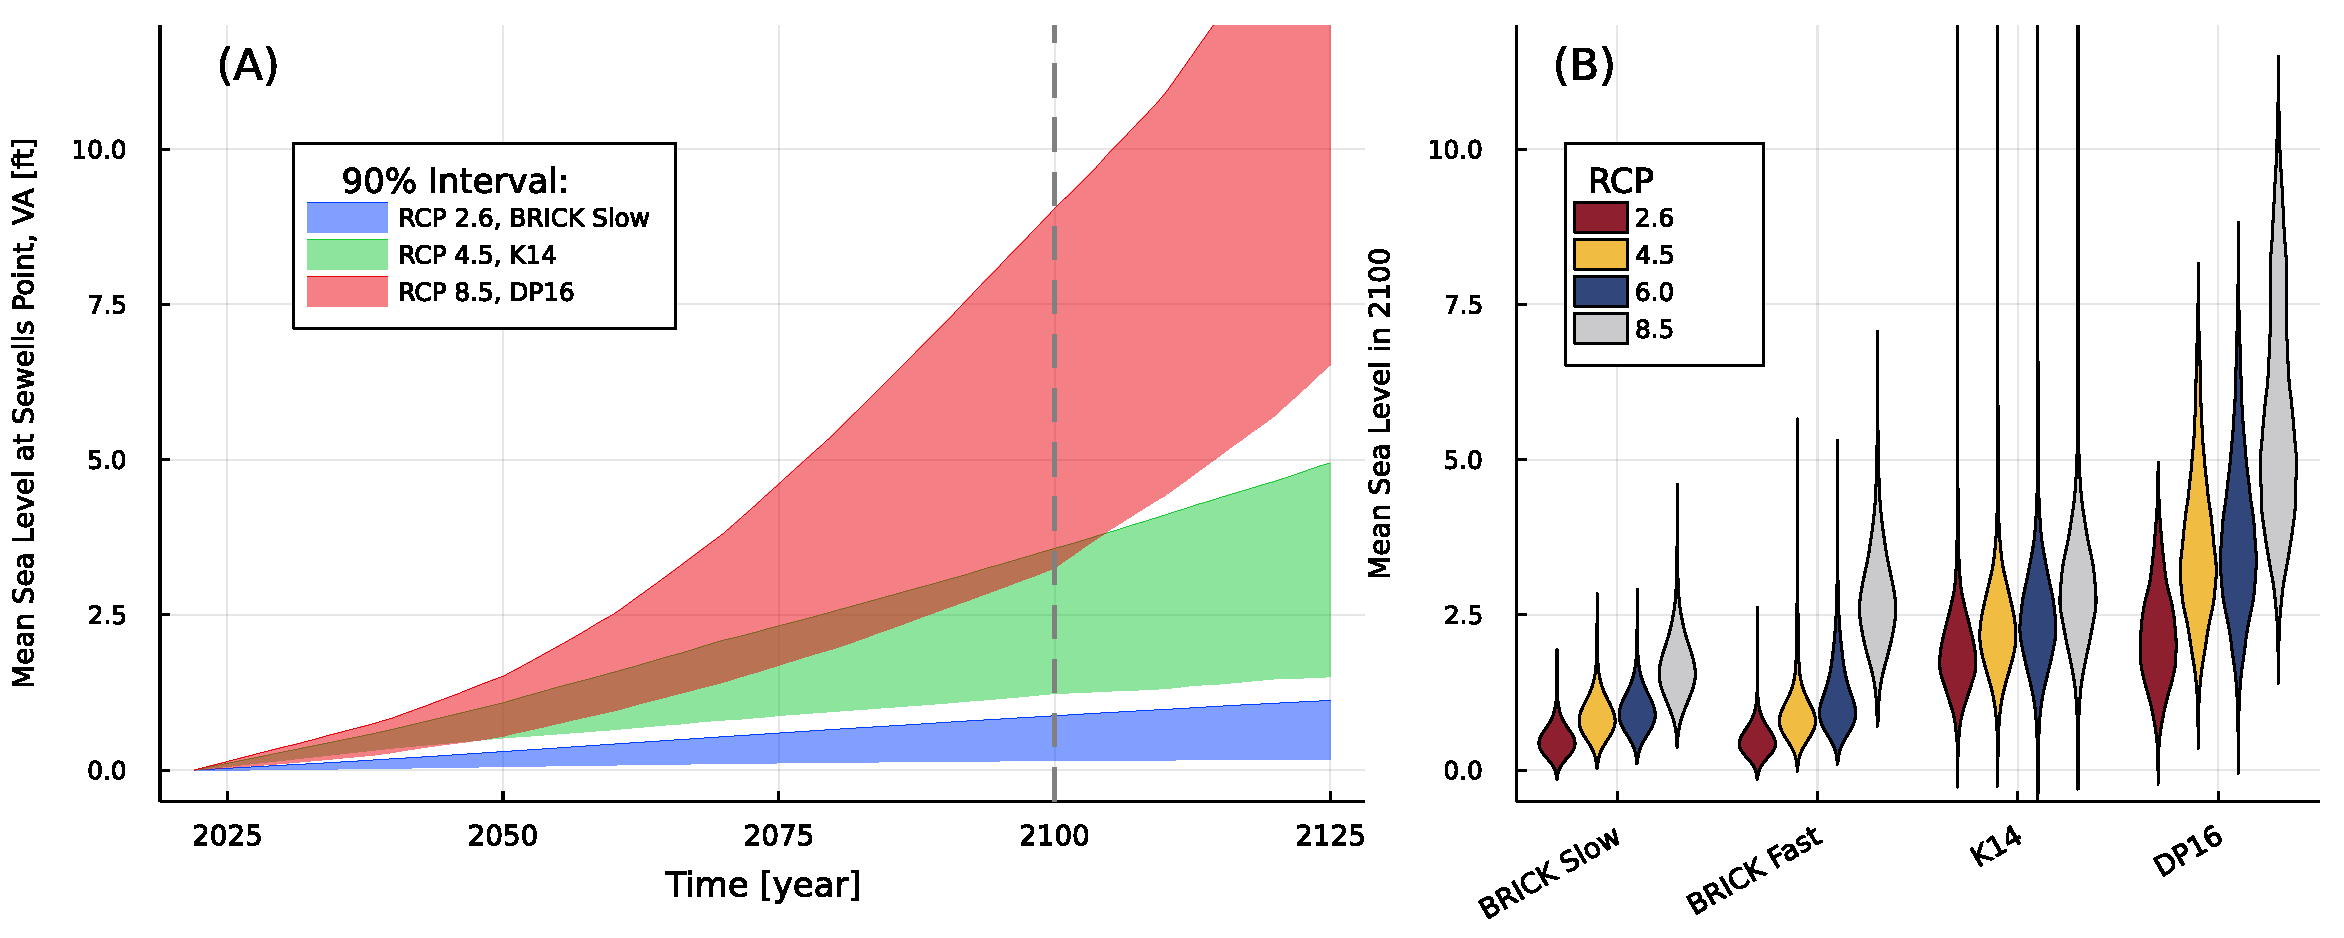
\includegraphics[width=\textwidth]{lsl-evolution}
    \caption{
        Projections of future mean sea level depend strongly on the choices of physical model and forcing.
        (A): 90\% confidence intervals for mean sea level at Sewells Point, VA as a function of time for a representative subset of three probabilistic models (out of sixteen).
        (B): probability distribution of \gls{msl} at Sewells Point, VA in the year 2100 for each probabilistic model considered.
    }\label{fig:lsl-evolution}
\end{figure}

The choices of physical model and \gls{rcp} scenario jointly determine future \gls{msl} $p(\overline{y}|t)$.
\Cref{fig:lsl-evolution}(a) shows the time-varying \glspl{pdf} of \gls{msl} for three representative models.
The divergence between the the best-case (blue) and worst-case (red) models is small in the early 21st century and increases rapidly thereafter.
\Cref{fig:lsl-evolution}(b) shows the \glspl{pdf} of mean sea level in 2100 (dashed vertical line in panel (a)) under each of the sixteen models considered.
We return in \cref{sec:multiple-pdf} to the problem that these multiple models poses to decision makers.

\subsection{Storm surges}\label{sec:storm-surge}

We model annual maximum floods $y(t)$ as the sum of sea level $\overline{y}(t)$ and annual maximum storm surges $y'(t)$.
In this subsection we describe the representation of storm surge in our model.

Data on storm surge comes from Sewells Point, VA (NOAA gauge 8638610).
The NOAA tides and currents dataset is freely available to the public at \url{https://tidesandcurrents.noaa.gov/waterlevels.html}.
Hourly recordings of water level are available from 1928 to the present; we use data from the period January 1, 1928 to December 31, 2021.
For each calendar year we first remove the annual mean, then extract the maximum water level.
We refer these maxima as the annual maximum storm surges $y'(t)$.

In the historical record, major surges have been driven by two different mechanisms: tropical cyclones and Nor'easters.
This time series of annual maxima is shown in \cref{fig:surge-obs-return}(a).
The largest recorded surge was the Chesapeake-Potomac hurricane of 1933, which caused a surge of over \SI{7}{ft} at this gauge, but other hurricanes and Nor'easters have caused surges above \SI{6}{ft}.

\begin{figure}
    \centering
    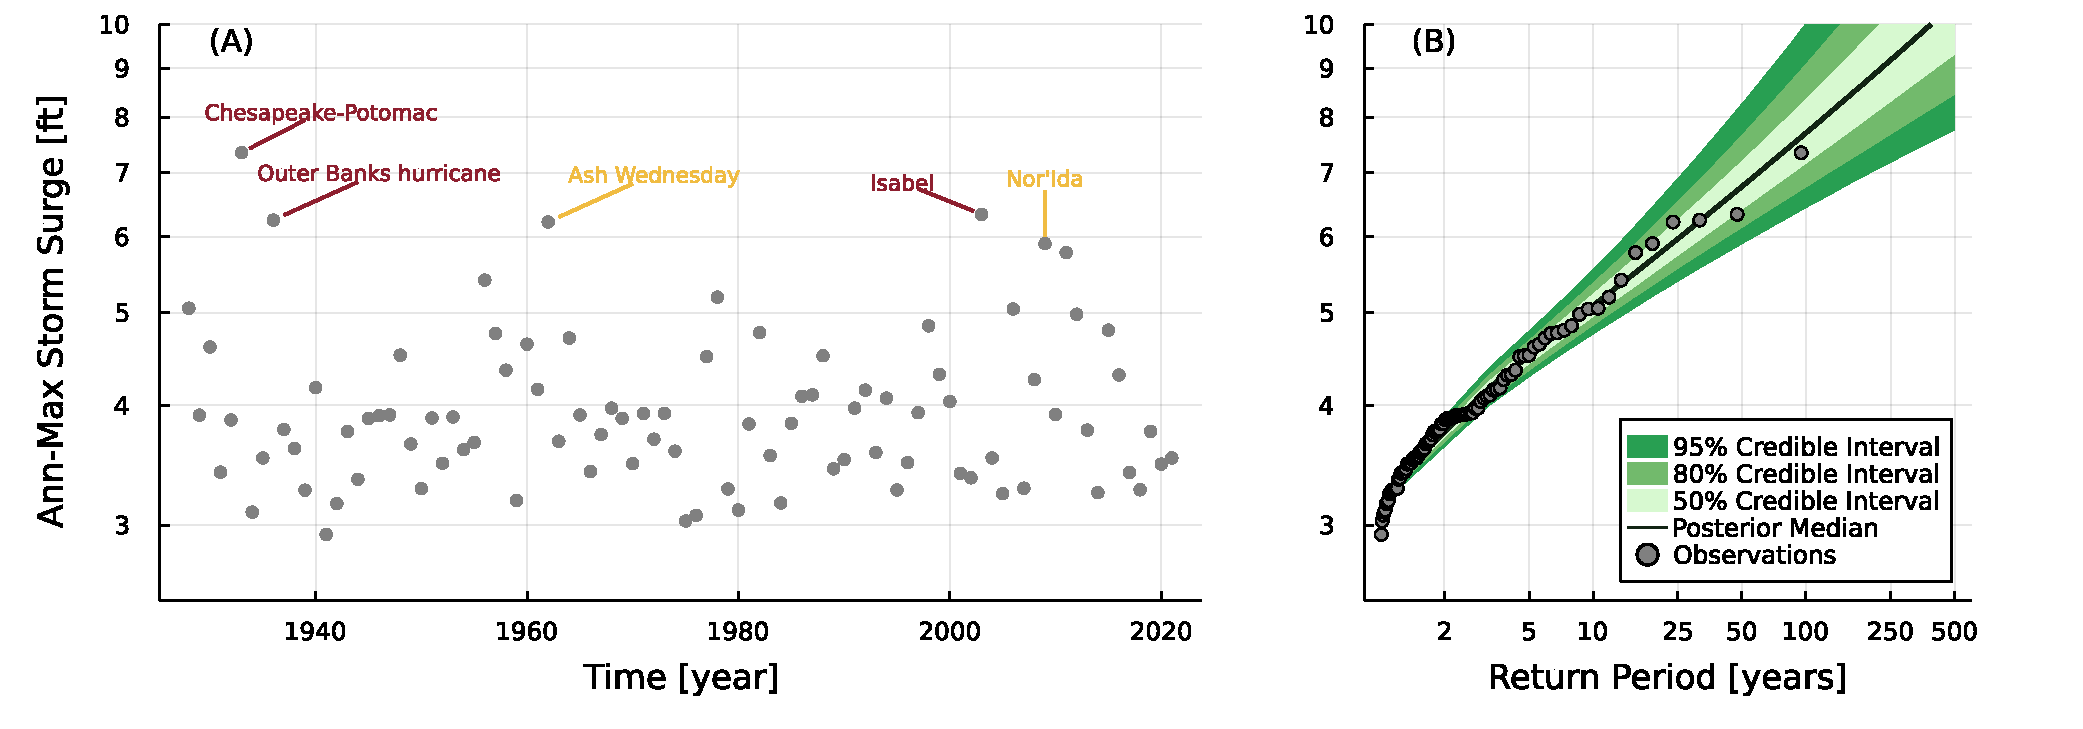
\includegraphics[width=\textwidth]{surge-obs-return}
    \caption{
        Annual maximum storm surges (after subtracting mean sea level) at Sewells Point, VA.
        (A):
        time series of historic storms.
        Red (yellow) arrows denote notable tropical cyclones (Nor'easters).
        (B):
        return periods.
        Dots indicate observed values; their $x$-value (``plotting position'') is calculated using the Weibull formula (eq.~\ref{eq:plot-pos}).
        Gray lines show the 50, 80, and 95\% posterior confidence intervals from the Bayesian \gls{gev} fit (\cref{sec:storm-surge}).
    }\label{fig:surge-obs-return}
\end{figure}

We model future storm surge using a stationary \gls{gev} model:
\begin{equation}\label{eq:surge-model}
    y'(t) \sim \text{GEV}\qty(\mu, \sigma, \xi),
\end{equation}
where $y'(t)$ is the storm surge (above sea level) in year $t$ and a \gls{gev} distribution with location $\mu$, scale $\sigma$, and shape $\xi$ has the probability density function
\begin{equation*}
    f(x | \mu, \sigma, \xi)= \begin{cases}
        \frac{1}{\sigma} \qty[ 1 + \qty( \frac{x-\mu}{\sigma} ) \xi ]^{-1 / \xi - 1} \exp \qty{- \qty[1+\qty(\frac{x-\mu}{\sigma}) \xi ]^{-1 / \xi} }, & \xi \neq 0 \\
        \frac{1}{\sigma} \exp \qty{-\frac{x-\mu}{\sigma}} \exp \qty{ -\exp \qty[-\frac{x-\mu}{\sigma}]},                                               & \xi=0.
    \end{cases}
\end{equation*}
This model assumes stationarity, neglecting any potential time dependence.

Our approach to model building follows a principled workflow for model building and checking \citep[see][for details]{gelman_workflow:2020}.
One model choice, analogous to the choice of statistical distribution or the assumption of stationarity, is the choice of how to represent prior information.
We include two forms of prior information.
First, we constrain $\xi > 0$ to reflect knowledge about the support of $y'$:
\begin{equation*}
    \mathrm{supp}~ y' =
    \begin{cases}
        \xi < 0: & y' \in \qty(-\infty,~ \mu - \nicefrac{\sigma}{\xi}) \\
        \xi > 0: & y' \in \qty(\mu-\nicefrac{\sigma}{\xi},~ \infty).
    \end{cases}
\end{equation*}
Since storm surges cannot be negative, only the latter is physically defensible.
This is related to the approach of \citet{martins_estimators:2000}, who use physical reasoning to place an informative prior $\xi$.
Second, we add weakly informative priors.
Rather than applying prior information directly over the joint distribution of the priors $\qty{\mu,\sigma,\xi}$, for which intuition may be difficult, we instead apply a prior over extreme quantiles of the distribution as in \citet{coles_evd:1996}.
Specifically we apply Normal (truncated at zero) priors over the 2, 10, 100, and 500 year return levels, with means \SIlist{4;6;10;15}{ft} and standard deviations \SIlist{1.5;1.75;2.25;2.75}{ft}, respectively.
These values were chosen to represent plausible physical ranges and are plotted in \cref{fig:surge-gev-priors}.

For inference, we draw \num{10000} samples from the posterior distribution $p(\mu,\sigma,\xi | y')$ using Hamiltonian Markov Chain Monte Carlo \citep{Betancourt:2017vd,hoffman_nuts:2011} implemented in the Turing package of the Julia programming language \citep{perkel_julia:2019,ge_turing:2018,tarek_dynamicppl:2020,besancon_distributions.jl:2021,bezanson_julia:2012}.
Diagnostics suggest (though cannot guarantee) convergence (see \cref{tab:surge-posterior-mcmc-diagnostics}).
We evaluate the model's fit using posterior predictive checks \citep[section 2.4 and references therein]{gelman_workflow:2020}.
Using the lag 1 and 2 partial autocorrelations, sample maximum, sample minimum, sample median, and Mann-Kendall test value as Bayesisan test statistics, we found that draws from the posterior predictive distribution matched the observed test statistic credibly (\cref{fig:surge-test-statistics}) although \cref{fig:surge-test-statistics}(b) suggests the possibility of temporal structure not captured by our stationary \gls{iid} model.
Future efforts could represent this structure by conditioning the parameters of the distribution on relevant climate indices \citep[as in][]{wong_structural:2020,Farnham:2016tw,farnham_jetstream:2017}.

\Cref{fig:surge-obs-return}(b) shows the estimated return periods for these storm surges.
The return period of the data (dots) is shown using the Weibull (``empirical'') plotting position
\begin{equation}\label{eq:plot-pos}
    \frac{r}{N + 1}
\end{equation}
where $N$ is the sample size and $r$ is the order of the $N$ observations ($r=1$ is the largest, $r=N$ is the smallest).
The good fit of the Bayesian fit (gray shading) to the data (points) suggest the modeling choices made are reasonable and sufficient for this didactic example.
Finally, a positive control test (\cref{fig:surge-synthetic-data-experiment}) validates the model's ability to recover known parameter values.

\subsection{Damages and metrics}\label{sec:ead-led}

The system model (``relationships'' in \cref{fig:xlrm}) is comprised of two key pieces.
The first is a fragility model that estimates the expected flood damages for a particular year (``expected annual damages''), given the elevation of the house and the mean sea level for that year.
The second converts model converts a time series of annual expected damages into lifetime expected damages.

We define expected annual damages in year $t$ as the expectation of the damage function with respect to storm surge.
This expectation depends on the house's height ($h = h_0 + \Delta h$) where $h_0$ is the initial height relative to the gauge and $\Delta h$ is the amount by which the house is elevated.
The expected annual damage is thus
\begin{equation}\label{eq:ead}
    \textrm{EAD}(t) = \mathbb{E}[D \qty(h-\overline{y}(t))] = \int_{y'} p(y') D \qty(h - \qty(\overline{y}(t) + y')) \dd{y'}
\end{equation}
where $D(h-y)$ is a deterministic function specifying damage as a function of flood depth (relative to the house).
Following \citet{zarekarizi_suboptimal:2020} we use the we use the Hazard U.S. (HAZUS) depth-damage curves provided by FEMA to parameterize $D(h-\overline{y})$; this depth-damage relationship is shown in \cref{fig:cost-depth-damage}.
For comparison, \cref{fig:cost-depth-damage} also shows results using the ``Europa'' depth-damage relationship developed by the Joint Research Center of the European Commission's science and knowledge service \citep{huizinga_depthdamage:2016}.
Although \citet{zarekarizi_suboptimal:2020} demonstrate that the choice of fragility function is important for informing house elevation, we use only the HAZUS model for simplicity.

The expected annual damage is sometimes calculated by assuming analytically tractable functional forms for the depth-damage relationship and for the  distribution of hazard \citep[\eg][]{vandantzig_dike:1956}.
However, the convolution of the HAZUS depth-damage equation with the \gls{gev} posterior does not have a tractable analytic solution so we instead estimate it through a Monte Carlo method (see \cref{sec:alg-ead} for details).
Then, because the expectation in \cref{eq:ead} depends only on $h-\overline{y}(t)$, we calculate expected annual damages for a wide range of possible values $h - \overline{y}(t)$ and use this to train a computationally efficient a surrogate model (see \cref{sec:surrogate-ead}).

The second component of the system model converts a time series of $\mathrm{EAD}$ into lifetime expected damages, which we define as the up-front  discounted sum of expected annual damages:
\begin{equation}\label{eq:led}
    \textrm{LED} = \sum_{t=t_i}^{t_f} \gamma^{\qty(t-t_i)-1} \textrm{EAD}(t),
\end{equation}
where the discount rate is $1 - \gamma$.
For the didactic purposes of this study we neglect uncertainty in the discount rate \citep{zarekarizi_suboptimal:2020,arrow_discount:2013} and use a fixed discount rate (see \cref{tab:uncertainties}).
We calculate lifetime expected damages \emph{for each \gls{sow} separately}.

To assess the performance of a given decision for a specific \gls{sow} (``Metrics'' in \cref{fig:xlrm}), we calculate the following metrics for each decision-\gls{sow} combination:
\begin{enumerate}
    \item ``Up-front cost'' is the cost of elevating a house. Following \citet{zarekarizi_suboptimal:2020}, we use estimates of construction cost from the Coastal Louisiana Risk Assessment \citep{fischbach_clara:2012}. We normalize this cost by house value. This cost curve is shown in \cref{fig:cost-up-front}.
    \item ``Lifetime expected damages'' is calculated following \cref{eq:led}.
    \item ``Expected lifetime costs'' is the sum of lifetime expected damages and up-front costs.\james{Make sure the figures all use this term}
\end{enumerate}

\subsection{Experiment design}

In the remainder of this article we incrementally develop a general framework, illustrated in \cref{fig:flowchart}, for analyzing climate risk management strategies under deep uncertainty.

Our framework considers $J$ \glspl{sow} $s_1, \ldots, s_J$ (here representing time series of \gls{msl}) and $I$ discrete decisions $x_1, \ldots, x_I$ (here representing the choice for how high to elevate the house).
For each combination of these, we calculate the vector of metrics described in \cref{sec:ead-led}, which we denote $u$.
Letting $f$ be a system model (here: the economic and engineering loss models in \cref{sec:ead-led}) we define $u_{ij} := f(x_i, s_j)$.

We begin in \cref{sec:exploratory} with an exploratory analysis (blue box in \cref{fig:flowchart}) that uses the system model to identify the conditions under which particularly desirable or undesirable outcomes occur.
This exploratory modeling does not require any assessment of the relative likelihood of the \glspl{sow}, but can only be interpreted as a ``what-if'' analysis.
We continue in \cref{sec:exploratory} with a scenario-conditional analysis (red box in \cref{fig:flowchart}) that integrates outcomes over all the \glspl{sow} corresponding to a particular model (here \gls{rcp} scenario and physical model structure).
While this analysis can be used to quantify the conditional distribution of outcomes, this conditional distribution will be different for each model considered.
We refer to this as ``the multiple \gls{pdf} problem.''
Finally in \cref{sec:synthesizing} we introduce a method for synthesizing uncertainty across the multiple \glspl{pdf} (orange box in \cref{fig:flowchart}) by weighting each \gls{sow}, given some subjective belief.

\begin{figure}
    \centering
    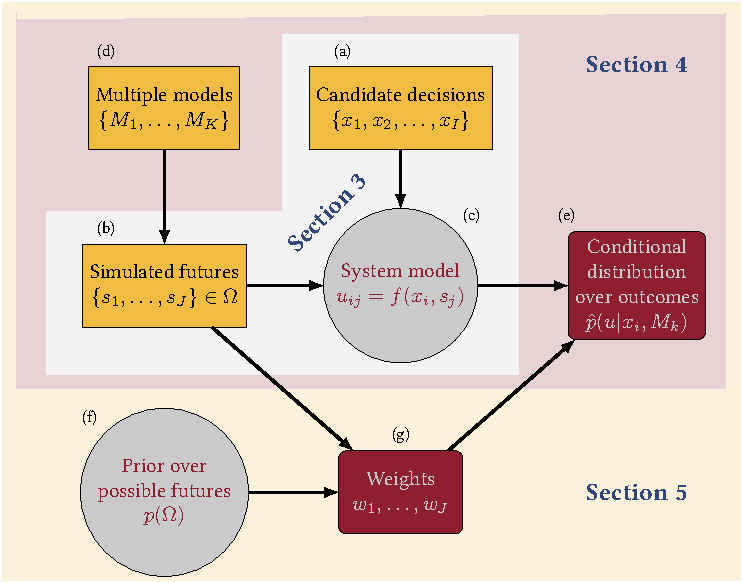
\includegraphics[width=\textwidth]{bayes-rdm.pdf}
    \caption{
        Outline of the proposed decision analytic framework.
        We begin in \cref{sec:exploratory} using a lens of exploratory modeling (region 1) to analyze the elevation problem.
        Next we use scenario-conditional optimization to illustrate the ``multiple \acrshort{pdf} problem'' (region 2).
        Finally we propose a method for weighting \glspl{sow} to synthesize uncertainties across multiple \glspl{pdf} (region 3).
    }\label{fig:flowchart}
\end{figure}

\section{Exploratory analysis}\label{sec:exploratory}

We begin by using our model in an ``exploratory'' mode with an aim of learning about interactions between system dynamics and decisions.
Exploratory modeling has been widely used in water resources management \citep{Brown:2012kb,Poff:2015jn,quinn_exploratory:2020,Steinschneider:2015kk}, analysis of coupled human-natural systems \citep{moallemi_exploratory:2020,moallemi_decisionsupport:2020}, and coastal adaptation \citep{sriver_sealevel:2018} and does not require any \emph{a priori} assessment of how likely a given \gls{sow} may be \citep{bankes:1993,kwakkel_exploratory:2013,reed_multisectordynamics:2022}.

\begin{figure}
    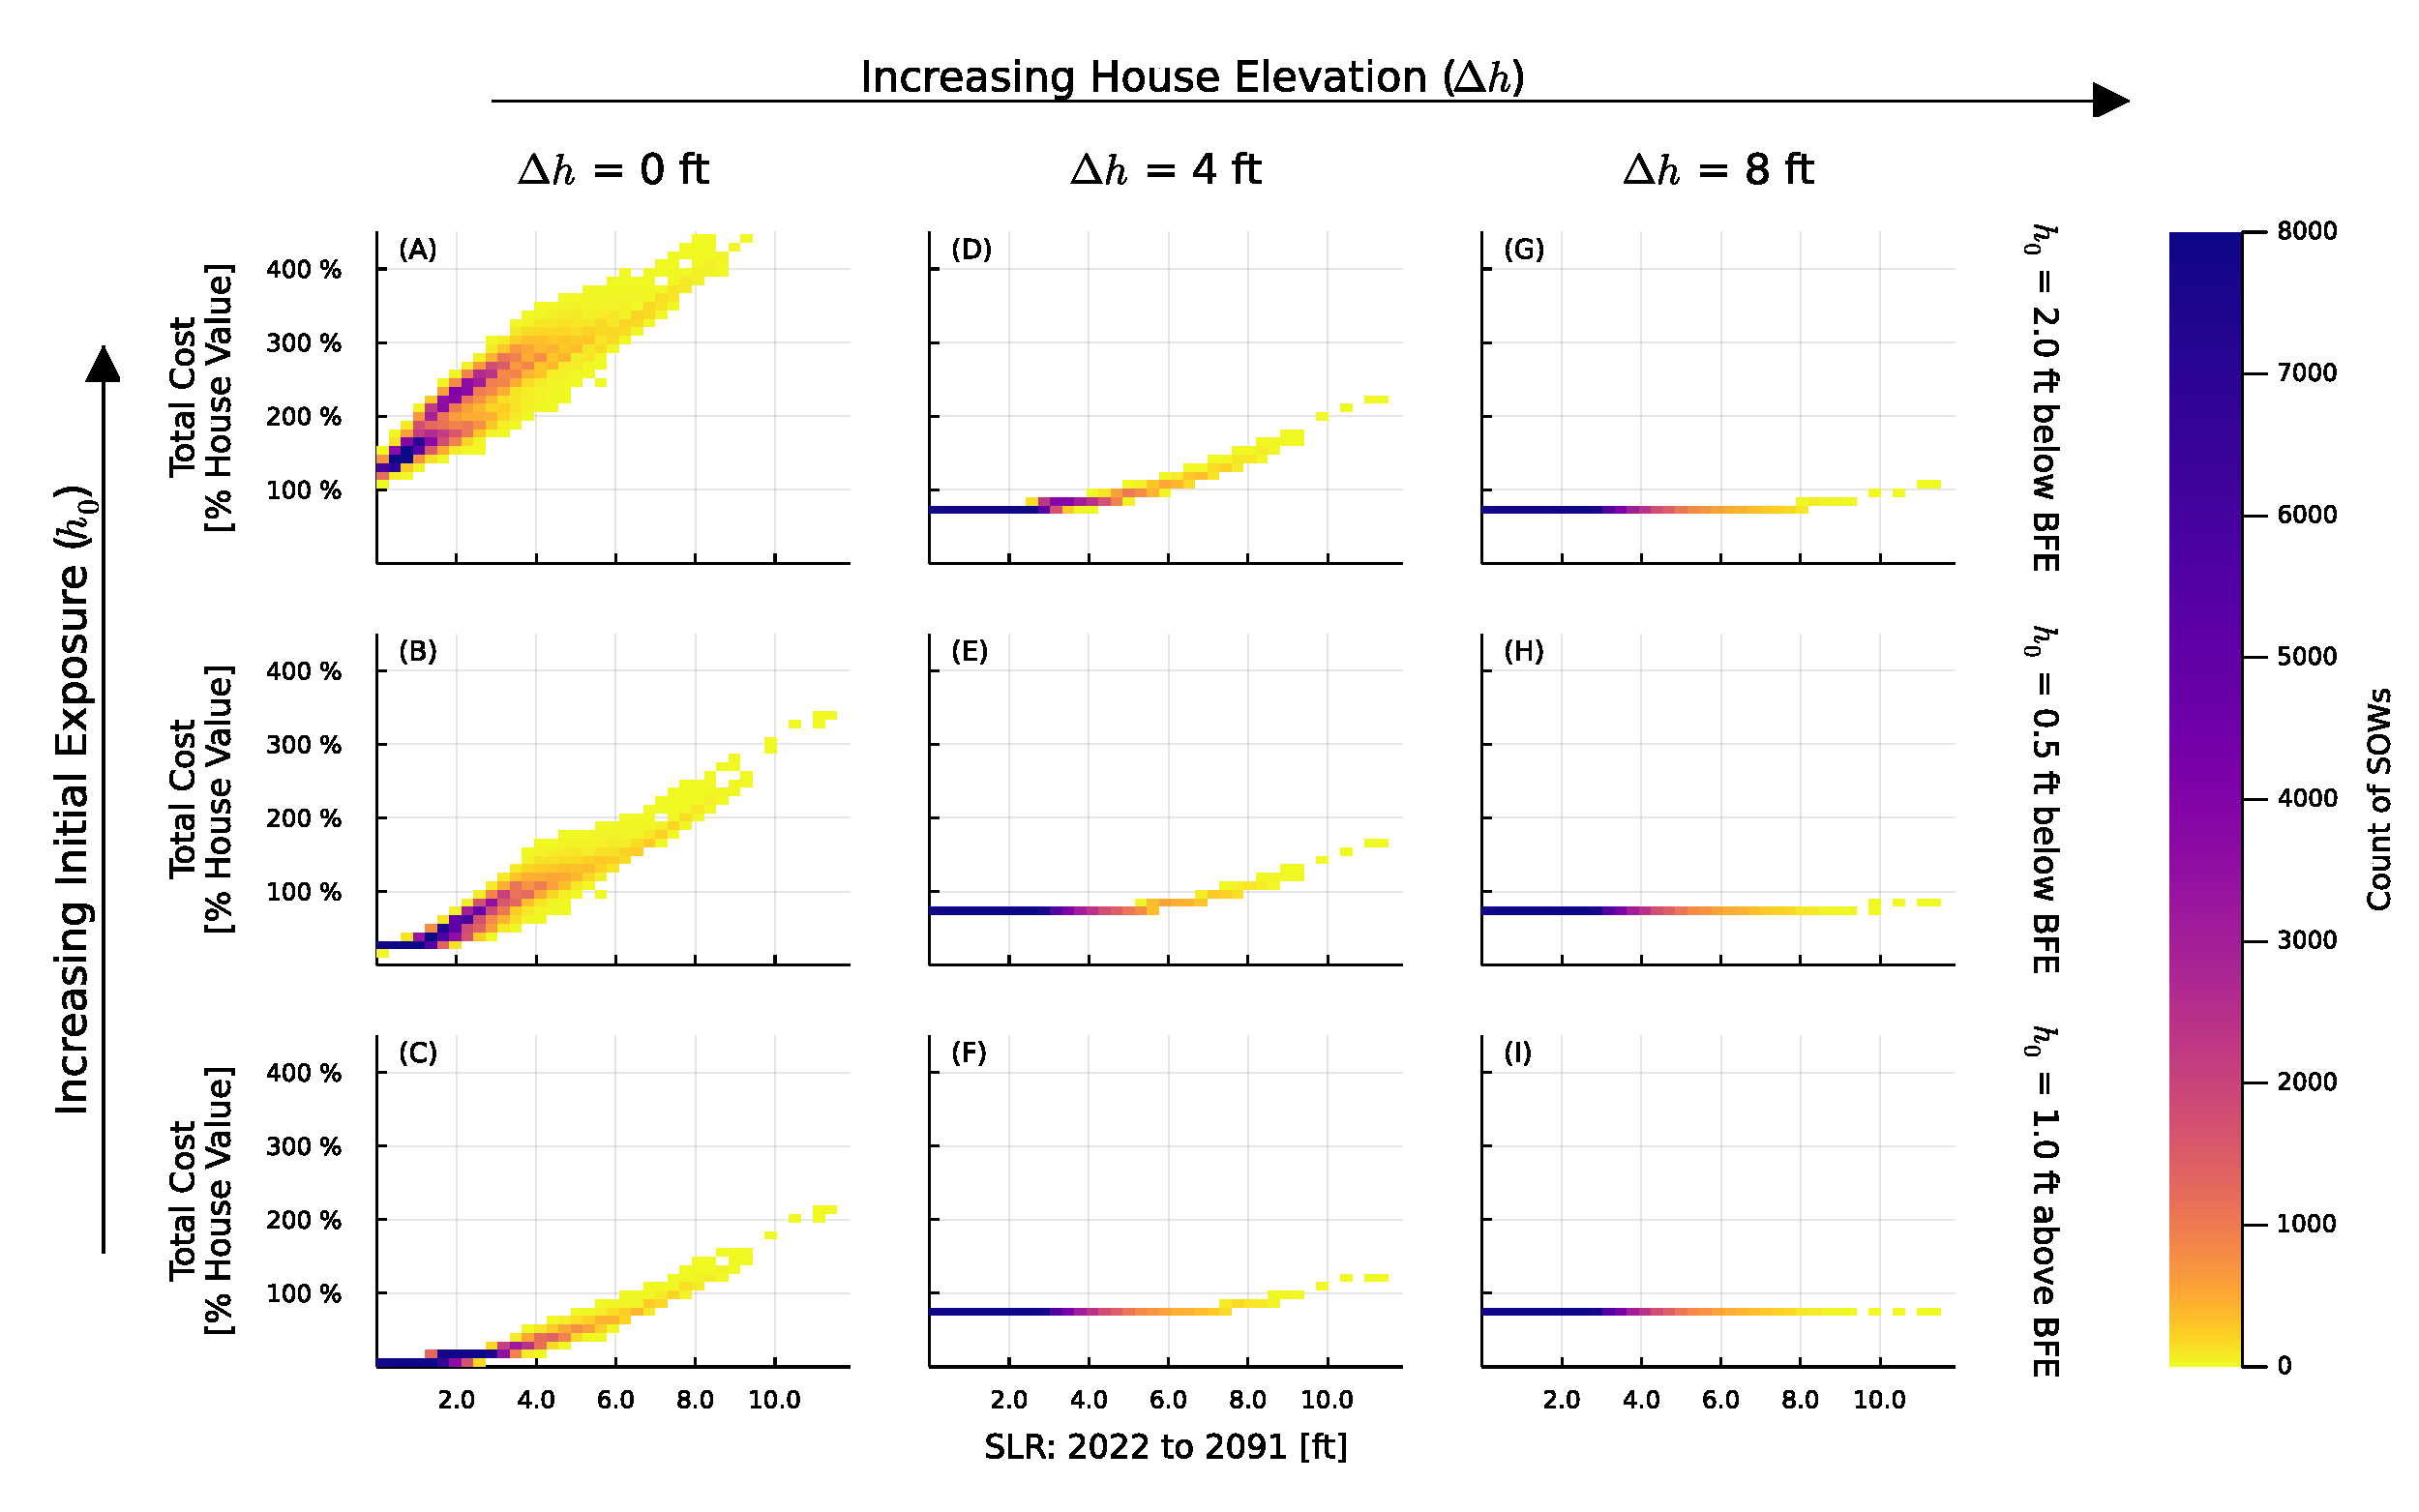
\includegraphics[width=\textwidth]{scenario-map-slr-cost}
    \caption{
        Scenario maps show the dependence of expected lifetime cost (damages plus up-front cost) as a function of \gls{msl} in 2100 for several values of $\Delta h$ and $h_0$.
        Colors indicate the density of \glspl{sow}; the color of each grid box corresponds to the number of \glspl{sow} falling within that box.
        The lowest-cost outcomes occur when both exposure is low ($h_0$ is large and \gls{slr} is minimal) and the house is not elevated (no up-front cost).
        The highest-cost outcomes arise when exposure is high ($h_0$ is small and \gls{slr} is rapid) and investment is inadequate.
        In all cases, elevating the house reduces the variance in total lifetime cost.
        Values are sensitive to model constants; see \cref{tab:uncertainties}.
    }\label{fig:scenario-map-slr-cost}
\end{figure}

\Cref{fig:scenario-map-slr-cost} shows the dependence of expected lifetime costs (damages plus up-front costs) as a function of height increase ($\Delta h$) and \gls{slr} over the house lifetime.
The best outcomes (yellow) arise when the house is not elevated ($\Delta h = 0$) and \gls{slr} is minimal (bottom left corners).
The worst outcomes (blue) arise when the house is elevated only slightly and \gls{slr} is rapid.
As $\Delta h$ increases, the best-case scenario becomes more expensive because up-front costs increase, but worst-case scenarios become less expensive because even if \gls{slr} is substantial, damages will be negligible.

This exploratory analysis can be used to quantify the regions of parameter space under which certain measure of performance are met \citep{herman:2015}.
For example, \cref{fig:scenario-map-height-slr} shows expected total costs as a function of $\Delta h$ and \gls{slr} from 2022-2092 for a single value of $h_0$.
As in \cref{fig:scenario-map-slr-cost}, for high values of $\Delta h$ the expected total costs are dominated by up-front costs, and are thus relatively insensitive to deep uncertainty in \gls{slr}.
However, for lower values of $\Delta h$ the expected total costs are highly sensitive to the modeled \gls{slr}.


Because this exploratory analysis makes no assumptions about the relative likelihood of different \glspl{sow}, no probabilistic conclusions can be drawn.
For example, while an analyst can report the fraction of \glspl{sow} that meet some criterion (often called a robustness metric), this fraction is in general highly sensitive to the strategy used to sample \glspl{sow} \citep{quinn_exploratory:2020} and the choice of robustness measure used \citep{mcphail_robustness:2019}, and may not correspond to the expected probability of this criterion being met in the future.
For this reason many analyses first use exploratory modeling to identify the conditions under which different decisions are optimal, then look to qualitative insight from models and expert judgement as to which scenarios are most likely \citep[\eg,][]{Brown:2012kb,Steinschneider:2015kk}.
To quantify this insight, however, a more formal approach is needed.\james{Revisit this wording perhaps}

\section{Scenario-conditional analysis: the multiple PDF problem}\label{sec:multiple-pdf}

In this section we build on the exploratory analysis of \cref{sec:exploratory} by aggregating insights across \glspl{sow} to quantify the probability distribution of outcomes, conditional on a particular model.
This probability distribution over outcomes can be used to quantify costs and benefits, map Pareto frontiers, or formulate optimal decisions.

To develop a set of \glspl{pdf}, we next interpret the available \glspl{sow} is as \gls{iid} draws from each of the sixteen models of \gls{slr}, as shown in \cref{fig:lsl-evolution}.
A formal notation is introduced in boxes (d) and (e) of \cref{fig:flowchart}: for each of $K=16$ models, we interpret all \glspl{sow} generated with that model as \gls{iid} draws from the distribution of outcomes.
We can then use this conditional distribution over outcomes to define metrics that depend only on the decision, such as averages or quantiles of outcomes.

\begin{figure}
    \centering
    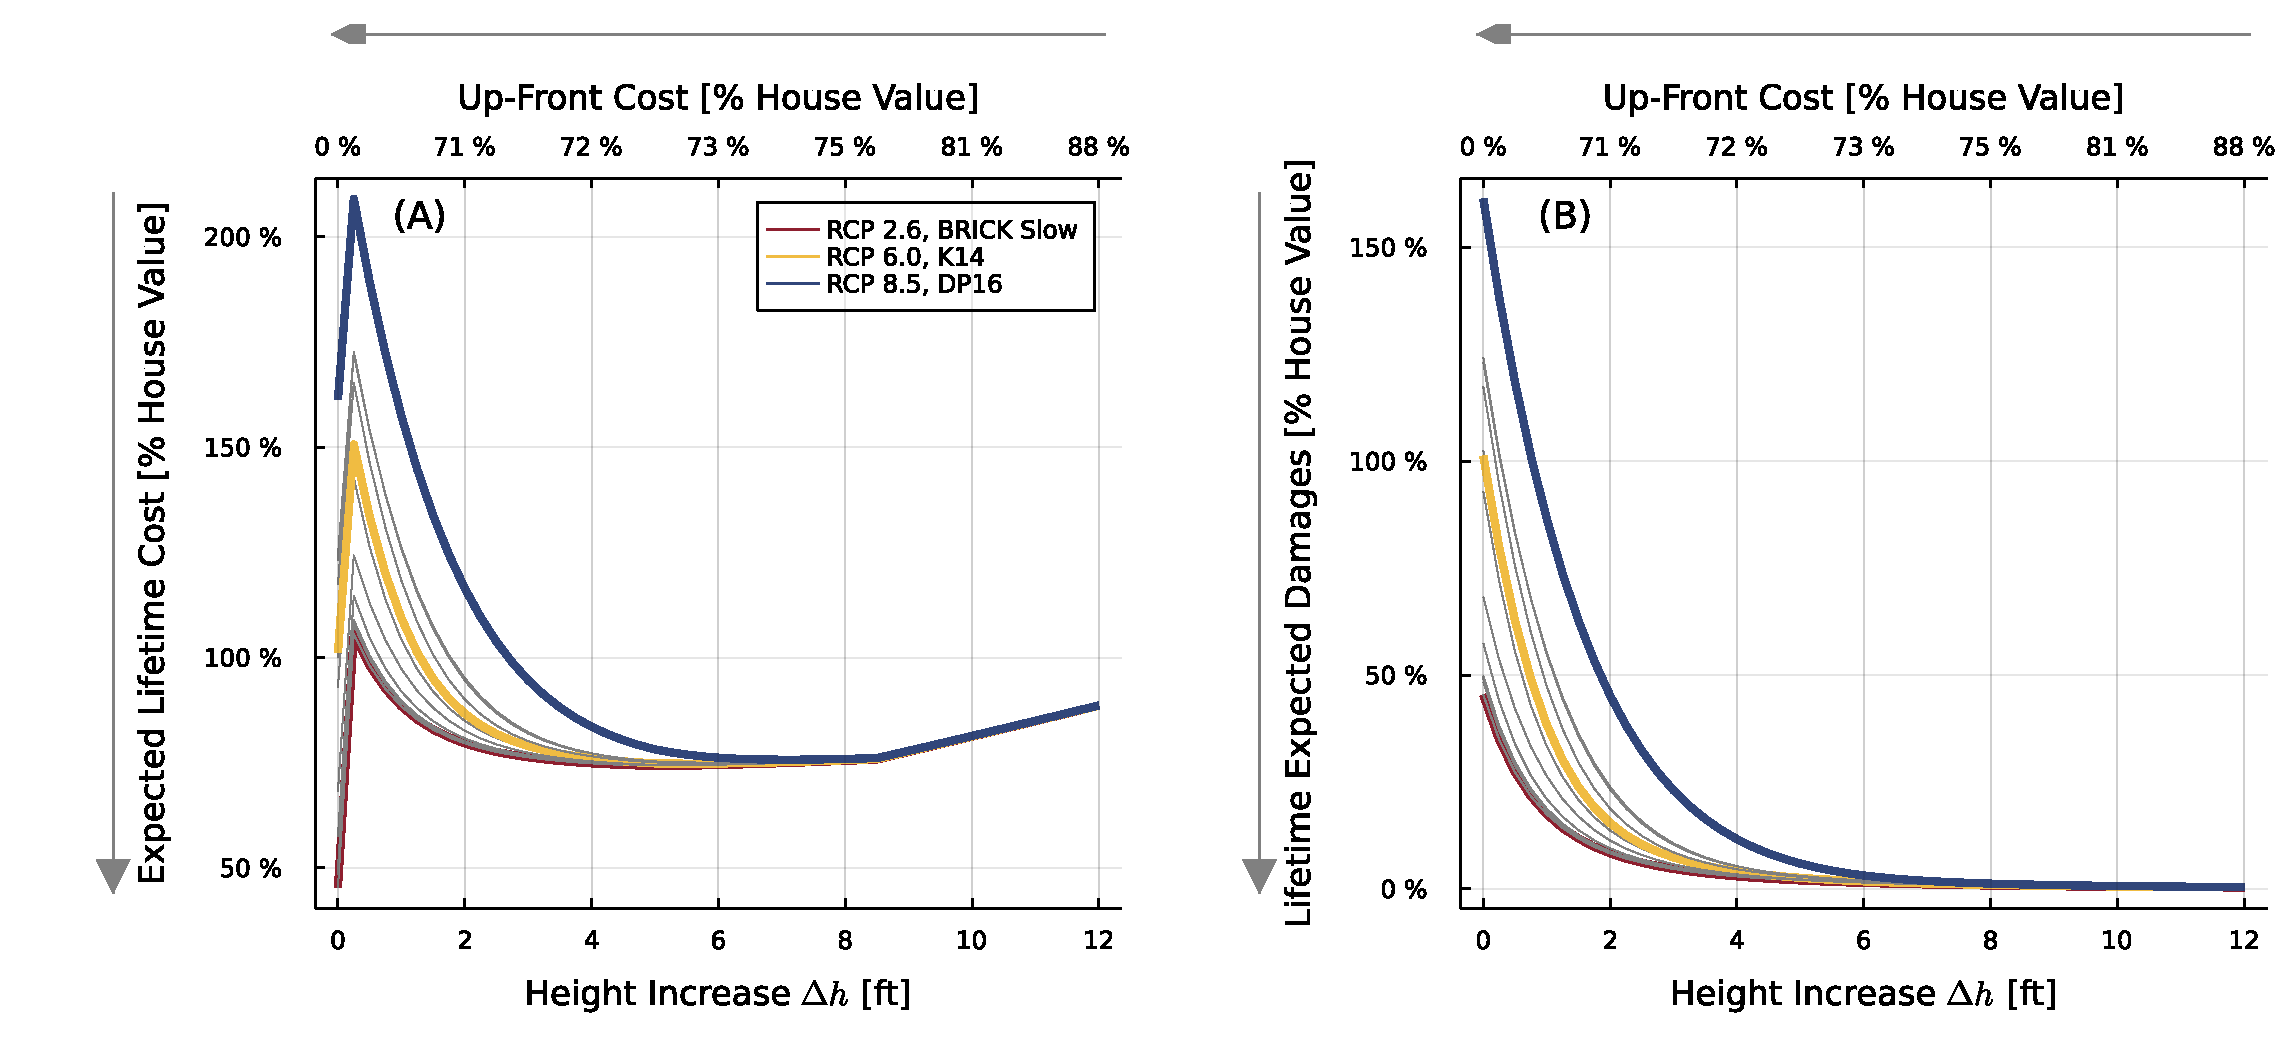
\includegraphics[width=\textwidth]{tradeoffs-by-rcp}
    \caption{
        Each probabilistic model or scenario leads to a different estimate of the Pareto frontier.
        (A): trade-off between up-front cost (which is a monotonic function of height increase) and expected lifetime costs.
        (B): trade-off between up-front cost and lifetime expected damages (eq.~\ref{eq:led}).
        Light gray lines show estimates for all 16 models (four \gls{rcp} scenarios times four physical parameterizations) considered.
        Colored lines highlight three representative models for emphasis.
    }\label{fig:tradeoffs-by-rcp}
\end{figure}

For example, \cref{fig:tradeoffs-by-rcp}(a) plots the total lifetime cost as a function of $\Delta h$ the sixteen models considered (three are highlighted).
Similarly, \cref{fig:tradeoffs-by-rcp}(b) plots the lifetime expected damages.
This figure shows that for small $\Delta h$, expected costs are low under optimistic models (\eg, \gls{rcp} 2.6 with slow ice sheet dynamics) and high under pessimistic models (\eg, \gls{rcp}8.5 with the DP16 model).
Consistent with \cref{fig:scenario-map-slr-cost}, the variability of lifetime costs decreases as $\Delta h$ increases.
Once $\Delta h$ reaches \SIrange[]{3}{7}{ft}, depending on the model considered, construction costs start to dominate flood losses, and thus higher values of $\Delta h$ increase average lifetime costs.

Calculating either of the quantities shown in \cref{fig:tradeoffs-by-rcp} requires synthesizing across \glspl{sow}.
However, these metrics are necessarily dependent on the model used (\ie, \gls{rcp} scenario and model of ice sheet dynamics).
This means that any assessment of decision performance (\eg, an optimal strategy, a Pareto frontier, or a cost-benefit analysis) is conditional upon an (explicit or implicit) model of future outcomes.
Where these models are implicit, they should be made more explicit to facilitate iterative model critique and improvement.

Second, this approach presents what we call ``the multiple \gls{pdf} problem'' because it leaves decision makers with many probability distributions from which to choose.
The multiple \gls{pdf} problem has been shown in other contexts.
For example, \citet{sharma_rcp:2021}\klaus{According to Earth's Future this is in fact 2021} modeled the reliability of stormwater infrastructure under different climate models and downscaling methods, finding diverging estimates of future rainfall hazard, even under a single \gls{rcp} scenario.\james{If we think of other examples let's put them here}

Although this scenario-conditional analysis is appropriate for understanding differences between models, its key limitation is that \emph{it places the burden for deciding which model to design for onto the end user.}
Further, once a model is chosen, it will under-represent total uncertainty, since this depends on both with- and between-model variability.

\section{Synthesizing PDFs for decision relevance}\label{sec:synthesizing}

\citet{schneider_scenarios:2002} criticized the reluctance of the \gls{ipcc} special report on emission scenarios \citep{nakicenovic_scenarios:2000} to assign probabilities to scenarios, writing ``if we in the scientific assessment business do not offer some explicit notions of the likelihood of projected events, then the users of our products -- policy analysts and policy makers -- must guess what we think these likelihood estimates are.''
In the context of climate risk management in general, and physical floodproofing of buildings in the coastal zone more specifically, an unwillingness to assign probabilities to \gls{rcp} scenarios defers to the end user (\ie, the homeowner, property manager, or local government) the choice of which scenario to design for.
Different end users will, in general, have different preferences that motivate different design choices given the same information, it is unlikely that these end users have expertise in global emissions pathways, climate sensitivity, or ice sheet dynamics.
Thus, motivated by the multiple \gls{pdf} problem illustrated in the previous section, we present here a framework for synthesizing information across multiple \glspl{pdf} using a subjective Bayesian interpretation of probability.

\subsection{Re-weighting}

Consider a set of \glspl{sow} $\qty{s_1, s_2, \ldots, s_j}$.
In general these \glspl{sow} may deliberately over-sample low-probability but potentially high-consequence futures, and so the distribution they are drawn from will not match our subjective belief about their true distribution, $p_\mathrm{belief}(\Omega)$.
To address this, we draw from approaches to sampling and poststratification.

First, we project the \glspl{sow} $s_1, \ldots, s_J$ onto a low-dimensional representation, which we denote $\psi_1, \ldots, \psi_J$.
This step is commonly used in \gls{abc} for the purpose of performing inference over parameters using a black-box model \citep[see][]{csillery_abc:2010}.
We take this low-dimensional statistic ($\phi$) to be \gls{slr} from 2022 to 2100, recognizing that future work could consider multidimensional summaries.

This projection simplifies analysis considerably by allowing us to define $p_\mathrm{belief}(\psi \in \Psi)$ instead of $p_\mathrm{belief}(s \in \Omega)$ as reasoning about a single quantity may be more straightforward than exploring a full probability distribution over time series.
Without loss of generality, we assume the $\psi_j$ to be sorted from least to greatest so that $\psi_{j-1} \leq \psi_j$, ($j \neq 1$).
Defining $F_\mathrm{belief}(s)$ to be the cumulative distribution corresponding to $p_\mathrm{belief}$, we calculate weights as illustrated in \cref{fig:grid-sketch}:
\begin{equation}\label{eq:weights}
    w_j = \begin{cases}
        j = 1     & F_\mathrm{belief}\qty(\frac{1}{2}\qty[\psi_1 + \psi_2])                                                                   \\
        1 < j < J & F_\mathrm{belief}\qty(\frac{1}{2}\qty[\psi_{j} + \psi_{j+1}]) - F_\mathrm{true}\qty(\frac{1}{2}\qty[\psi_{j-1} + \psi_j]) \\
        j = J     & 1 - F_\mathrm{belief}\qty(\frac{1}{2}\qty[\psi_{J-1} + \psi_J]).
    \end{cases}
\end{equation}

TODO\james{This paragraph needs some work}
The key point to get across is what a subjective belief means in the Bayesian context \citep{savage:1954,gelman_philosophy:2013,gelman_subjectiveobjective:2017}.
David Spiegelhalter had a nice comment on a podcast where he explained that in medicine, there isn't a ``true'' probability that, for example, you will get cancer; this is not some real quantity that can be measured \citep[hence the famous ``probability isn't real'' admonisment of][]{definetti_probability:1972}.
Similarly, the probability distribution of \gls{slr} in 2100 isn't something that can be measured.
However, probability provides a clear and self-consistent mathematical language for reasoning about uncertainty, which is why we're using it.
A key advantage is that \textbf{since we can't be right, we can at least be transparent} about the assumed values of sea level in 2100, rather than hiding behind implicit assumptions.
Thus we refer to the $M_k$ here as \emph{priors} to reflect that they consistently represent our current knowledge.

\begin{figure}
    \centering
    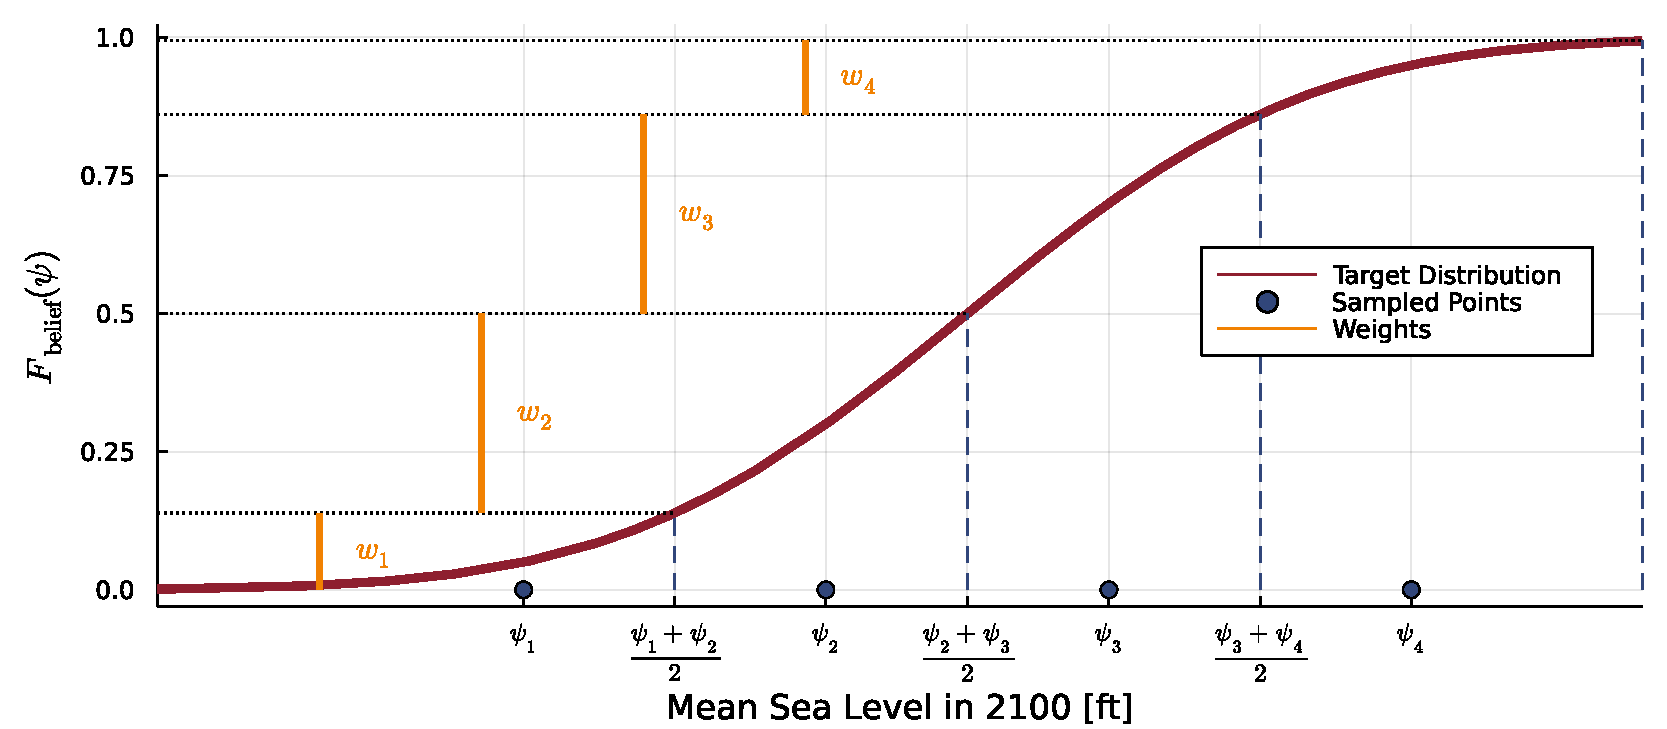
\includegraphics[width=\textwidth]{grid-sketch}
    \caption{
        Schematic of \gls{sow} weighting scheme defined in \cref{eq:weights} for $J=4$.
        This method is illustrated for a hypothetical target distribution (orange line) and four samples $\psi_1, \psi_2, \psi_3, \psi_4$ (blue dots).
        As shown in \cref{eq:weights}, the weights $w_j$ (vertical blue lines) are calculated based on the \gls{cdf} of the target distribution at the halfway points $\frac{1}{2}\qty[\psi_i+\psi_{i+1}]$ (vertical dashed lines).
    }\label{fig:grid-sketch}
\end{figure}

\subsection{Expert assessment}

We construct two probabilistic models for $p_\text{belief}$, based on expert assessments published by \gls{noaa}.
Following \citet{fuller_inversion:2017}, we convert published ranges into Normal probability distributions by interpreting the bounds of the published range as $\pm 2$ standard deviations from the mean.
\begin{enumerate}
    \item Table~2.4 of \citet{sweet_slr:2022} provides a range of \gls{slr} scenarios for different regions of the country; for the Northeast this range is \SIrange{0.6}{2.1}{\meter} (\SIrange{2.0}{6.9}{ft}) for the low and high scenarios, respectively. These ranges closely those of \citet{pfeffer_sealevel:2008} used in \citet{fuller_inversion:2017}. We refer to this model for $p_\text{belief}$ as ``All \gls{ssp}.''
    \item \Cref{fig:lsl-evolution} indicates that the highest (lowest) sea level rises occur under \gls{rcp} 8.5 (2.6), which are unlikely under current global pathways \citep{hausfather_scenarios:2020}. Table~2.4 of \citet{sweet_slr:2022} gives projections of total \gls{slr}, relative to a 2005 baseline under different \glspl{ssp}. Discarding \gls{ssp} 1 (corresponding to \gls{rcp} 2.6) and \gls{ssp} 5 (corresponding to \gls{rcp} 8.5), a plausible range of \SIrange{0.4}{0.92}{\meter} (\SIrange{1.3}{3.0}{ft}) is given. We refer to this model for as ``Likely SSPs.''
\end{enumerate}
\Cref{fig:lsl-priors-weights}(A) shows a visual representation of the models for $p_\text{belief}$ in panel.

A practical advantage of our weighting method (\cref{eq:weights}) is that changing the weights does not require re-sampling the \glspl{sow} or recomputing outcomes.
Thus it is computationally cheap to perform robustness checks that compare the effect of different weighting schemes


\subsection{Implications}

A few sentences explaining this trade-off curve\ldots\james{Add more}
Notably, they give different guidance.
If $p_\text{belief}$ is based on all \glspl{ssp}, elevating the house by approximately \SI{6}{ft} saves approximately 15\% of the house value relative to not elevating.
Conversely if $p_\text{belief}$ is based on the likely \gls{ssp} scenarios, then elevating the house costs approximately 15\% of the house value relative to not elevating.
Comparing the colored lines that synthesize uncertainty to the gray lines that consider a single scenario indicates the importance of integrating across uncertainties.

\begin{figure}
    \centering
    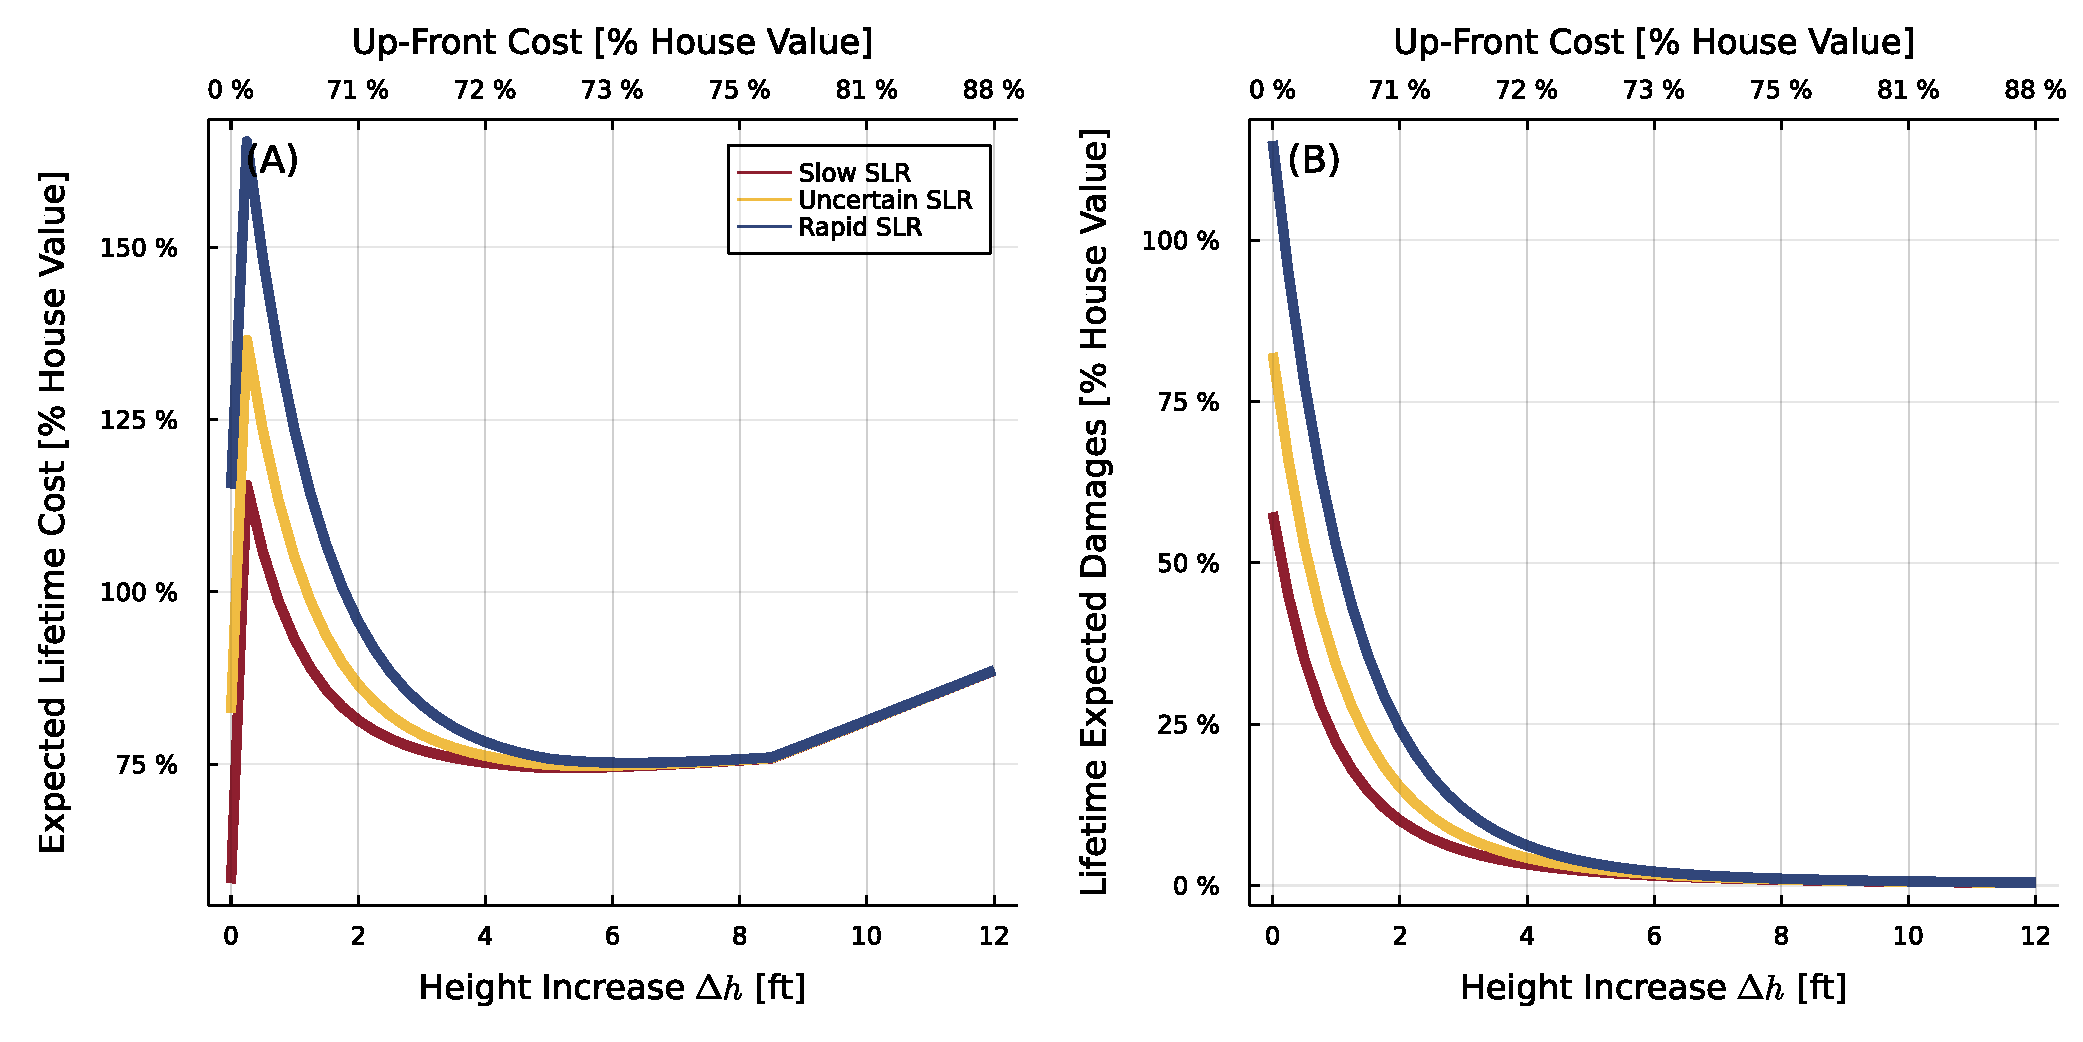
\includegraphics[width=\textwidth]{tradeoffs-by-prior}
    \caption{
        As \cref{fig:tradeoffs-by-rcp}, but Pareto frontiers are shown for the full distribution of outcomes, for two models of $p_\text{belief}$ (colors).
        Thin gray lines show the trade-off curves for each \gls{rcp} scenario and model separately as in \cref{fig:tradeoffs-by-rcp}.
    }\label{fig:tradeoffs-by-prior}
\end{figure}

This technique can also be used as a diagnostic tool\ldots\james{To do}
Specifically: what would I need to believe in order to justify some assumption?

\begin{figure}
    \centering
    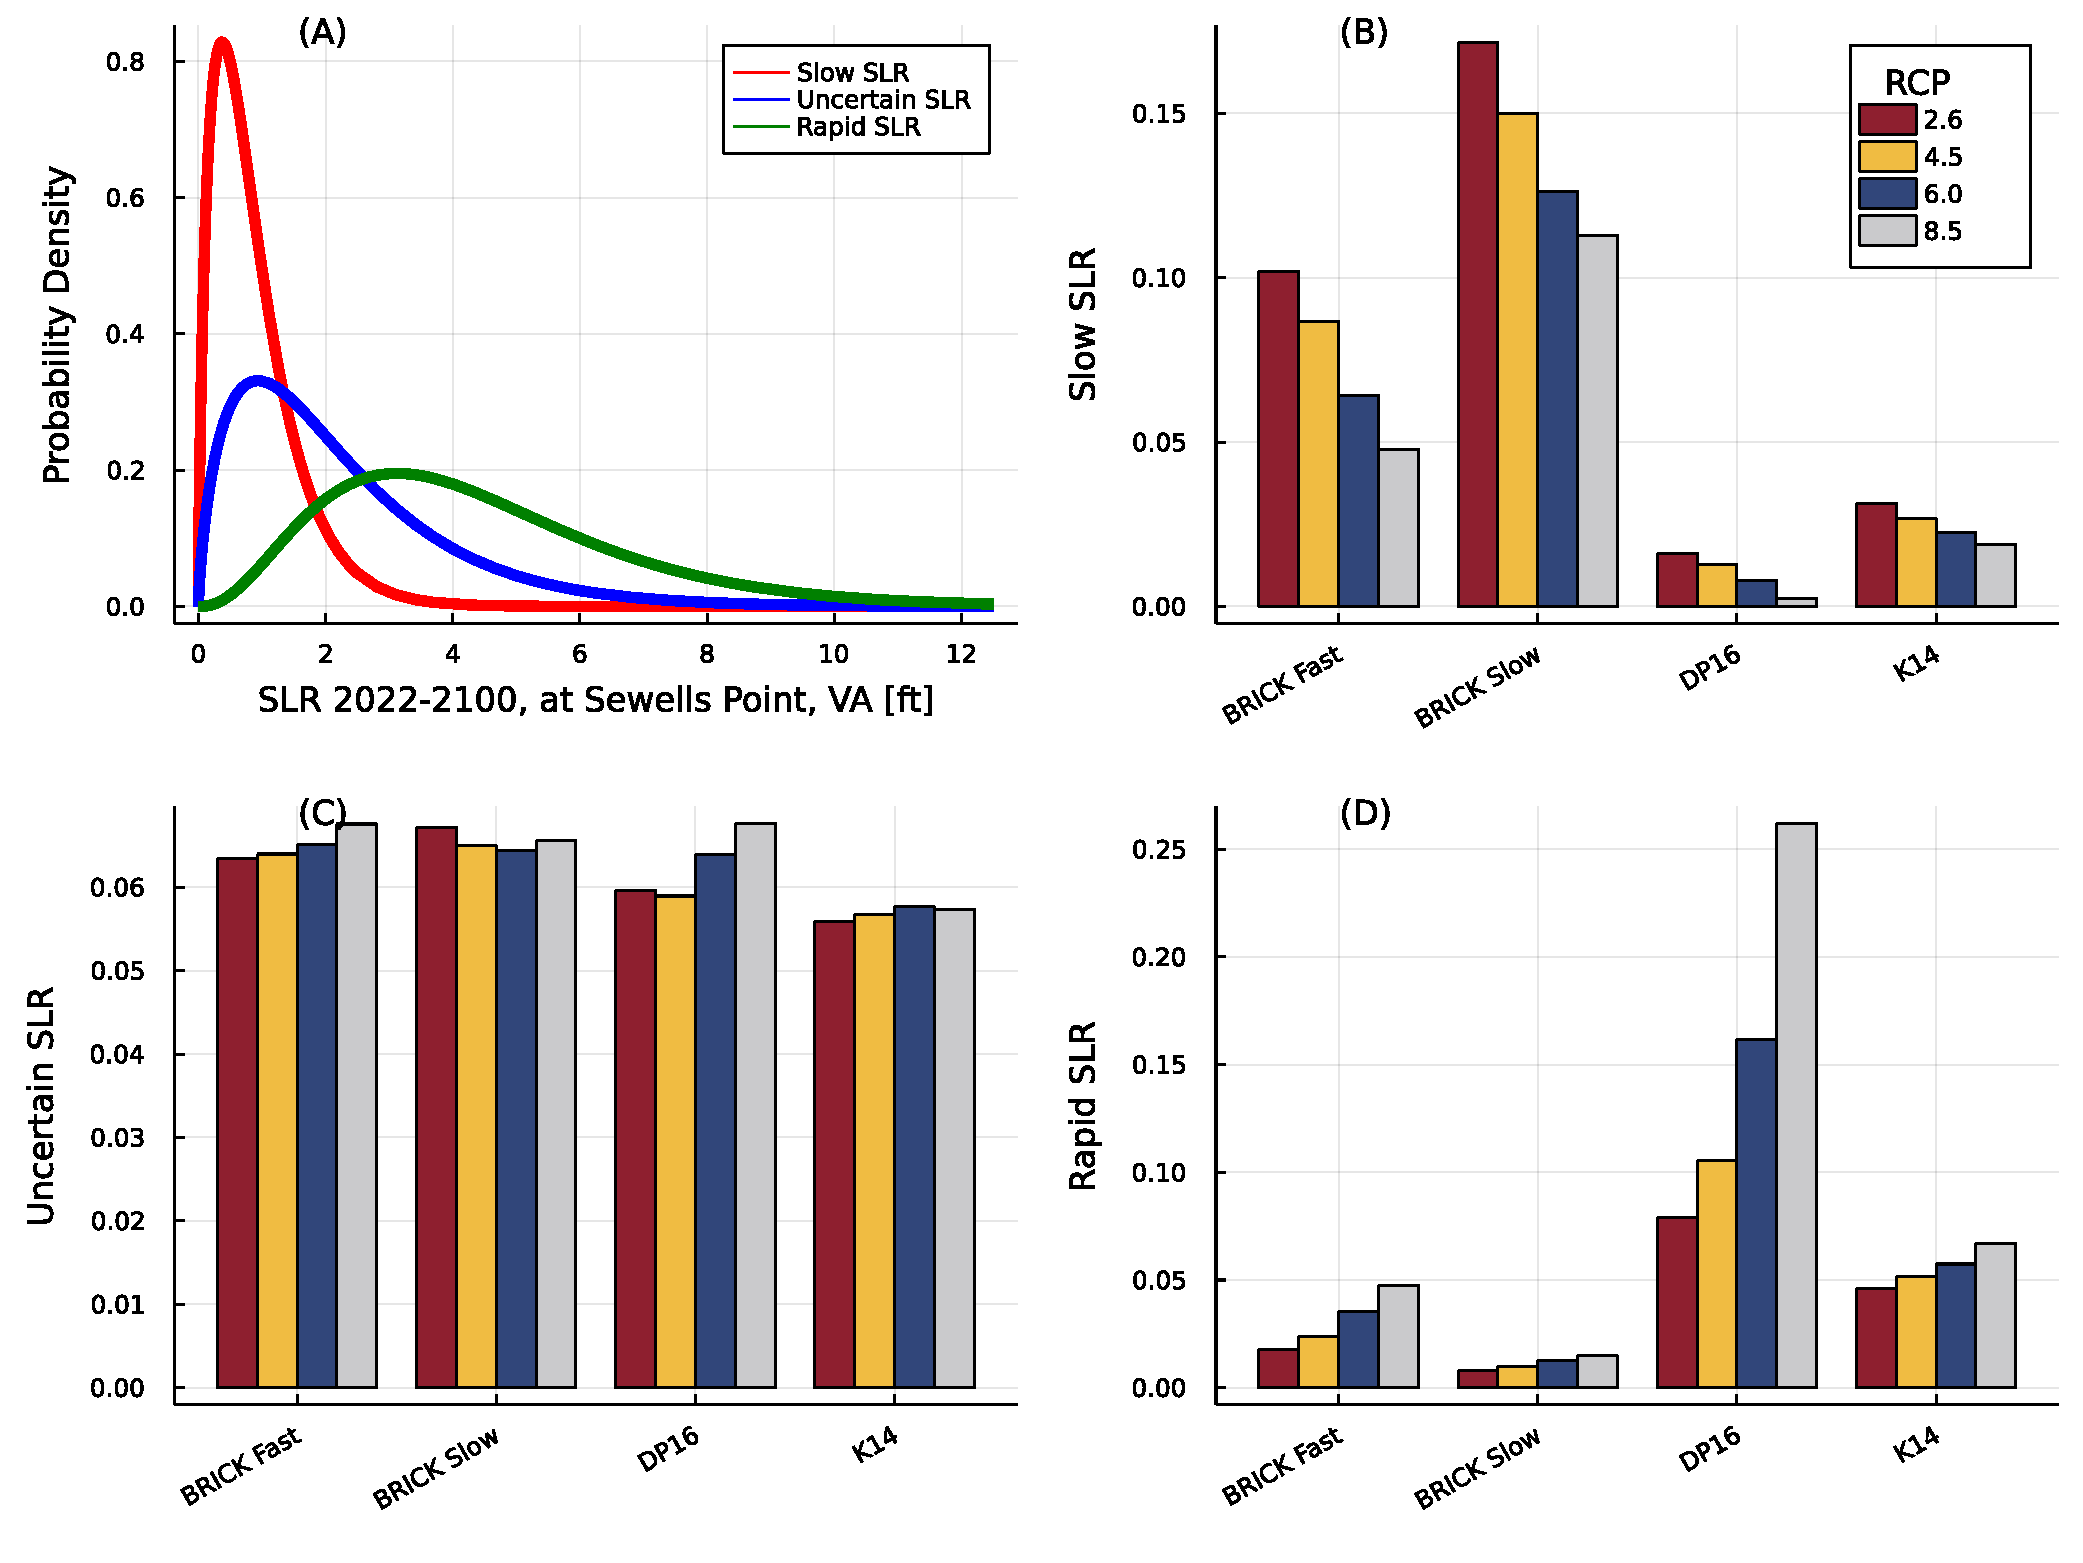
\includegraphics[width=\textwidth]{lsl-priors-weights}
    \caption{
        Subjective priors for local sea level.
        We develop two distributions (``subjective priors'') representing plausible probabilistic beliefs about \gls{msl} at Sewells Point, VA in 2100, relative to the present.
        The \glspl{pdf} of these subjective priors are shown in panel (A).
        In panels (B-C) we show the relationship between these subjective priors and the 16 probabilistic models (four \gls{rcp} scenarios and four physical representations) available.
        Specifically, (B-C) show the average weight given to each model by each of the subjective priors.
    }\label{fig:lsl-priors-weights}
\end{figure}


\section{Discussion and conclusions}\label{sec:conclusions}

Quick summary of what our motivation was
\begin{enumerate}
    \item Explore every \gls{sow}
    \item Be transparent about how we are calculating trade-offs
    \item Work with existing physical model ensembles
\end{enumerate}
Quick summary of what we have done
\begin{enumerate}
    \item Will fill in.
\end{enumerate}

\subsection{Limitations and future work}

Limitations of the re-weighting
\begin{enumerate}
    \item Our prior $p(\Omega)$ is limited -- we are just using \gls{msl} in 2100 but we could be looking at more parameters of it including rate of change, \etc
    \item The real world is in a state of ``unknown unknowns'' \citep[level 5 as defined in][fig.~1]{walker_deep:2013} so trying to represent \emph{all} uncertainty is futile; we must make subjective modeling choices and assumptions about what is most important
    \item The Uniform and Normal approaches used in \citet{fuller_inversion:2017} were applied for their simplicity and interpretability, but we note that they may not represent a fully calibrated prior belief about \gls{slr}; we refer the reader to \citet{gelman_workflow:2020} for a discussion of model checking steps that be applied.
\end{enumerate}
Limitations of the case study
\begin{enumerate}
    \item Objectives: real people might care about uncertainty (risk aversion), probability of experiencing flooding at all (disruptions are hard to quantify), usable space created under the house, and more
    \item More uncertainty (damage functions, cost of construction, lifespan, discount rate, \etc)
    \item Better data on cost of elevation and depth-damage
    \item Scalability: optimize separately for different kinds of house structures and locations
    \item Timing
    \item More physics -- we neglect hydrodynamics and tides
\end{enumerate}
Future research needs:
\begin{enumerate}
    \item This didactic example illustrates a need for better synthesis and communication of deep uncertainties for decision making.
    \item More complex models to capture more relevant metrics
    \item Better models of nonstationary hazards
    \item Interacting, sequential decisions
\end{enumerate}

\subsection{Policy relevance}

This approach can be used in many other contexts
\begin{enumerate}
    \item Stormwater management \citep{sharma_rcp:2021,lopez-cantu:2018}
    \item Levee heightening \citep{garner_slrise:2018,oddo_coastal:2017,vandantzig_dike:1956}
    \item Lots of economic models like social cost of carbon or effect of policy on metrics of interest make assumptions about deep uncertainties!\james{Let's emphasize this -- really important to policy analysis under deep uncertainty}
    \item Model structure uncertainties
    \item Local government revenues are sensitive to flood losses; this approach can be used to structure updates to building codes \citep{shi_municipal:2020}
\end{enumerate}
Key summary about the importance of integrating across uncertainties

\section*{End Matter}

\subsection*{Acknowledgements}

This work was supported by \acrfull{noaa} through the Mid-Atlantic Regional Integrated Sciences and Assessments (MARISA) program under NOAA grant NA16OAR4310179 and by the Penn State Center for Climate Risk Management.
JDG thanks Rice University for support.
KK thanks Dartmouth College for support.
The authors thank Tor Erlend Fjelde for helpful comments.

\subsection*{Code and data availability}

All code, including source code, is available under the GNU Public License (version 3) at \url{https://github.com/jdossgollin/2021-elevation-robustness}.
This code is written in the open source Julia programming language.

\subsection*{Author Contributions}

JDG and KK designed the research.
JDG wrote the codes and ran simulations.
JDG wrote the manuscript in consultation with KK.
JDG and KK revised the manuscript.

\printbibliography

\appendix
\newcommand{\hbAppendixPrefix}{S}
\renewcommand{\thefigure}{\hbAppendixPrefix\arabic{figure}}
\setcounter{figure}{0}
\renewcommand{\thetable}{\hbAppendixPrefix\arabic{table}}
\setcounter{table}{0}
\renewcommand{\theequation}{\hbAppendixPrefix\arabic{equation}}
\setcounter{equation}{0}

\newpage
\section{Supplemental methods}

\subsection{Algorithm to estimate expected damages}\label{sec:alg-ead}

\begin{enumerate}
    \item For $k=1, \ldots, K$:
          \begin{enumerate}
              \item sample a draw from the posterior distribution of flood hazard to get $\qty{ \mu_k, \sigma_k, \xi_k }$
              \item simulate a single storm surge from the stationary distribution (\cref{eq:surge-model}) and add the mean sea level to get total flood depth $y^\mathrm{sim}_k$
              \item calculate the flood damages for this draw by plugging the annual maximum flood depth ($h - y_k$) into  the deterministic HAZUS depth-damage relationship, storing this as the $k$th damage.
          \end{enumerate}
    \item Estimate expected annual damages as the sample mean of the $K$ estimates
\end{enumerate}

\subsection{Surrogate model for expected annual damages}\label{sec:surrogate-ead}
Evaluating expected annual damages for each of $N$ simulations of \gls{slr}, each of $J$ draw from the posterior distribution of storm surge, and each of $T$ time steps requires $N \times J \times T \times K$ simulations.
Since $K$ must be large in order to accurately approximate the integral, this requires incurring a heavy computational cost.
However, noticing that this function depends only on the elevation of the house relative to \gls{msl}, we develop a simple emulator for expected annual damages given this difference: $\hat{D}(h - \overline{y})$.
To do this, we  precompute expected annual damage for all height differences in \SI{0.25}{ft} increments from \SIrange{-30}{30}{ft} and fit a piecewise linear interpolation to this data.
We use $K=\num{1e6}$ samples to fit this emulator for each of the 241 increments.
This model is shown in \cref{fig:cost-expected-damage-emulator}.
Once this interpolation has been precomputed, calculating expected annual damage for a particular year only requires evaluating a piecewise linear function.

\section{Supplemental figures}

\begin{figure}
    \centering
    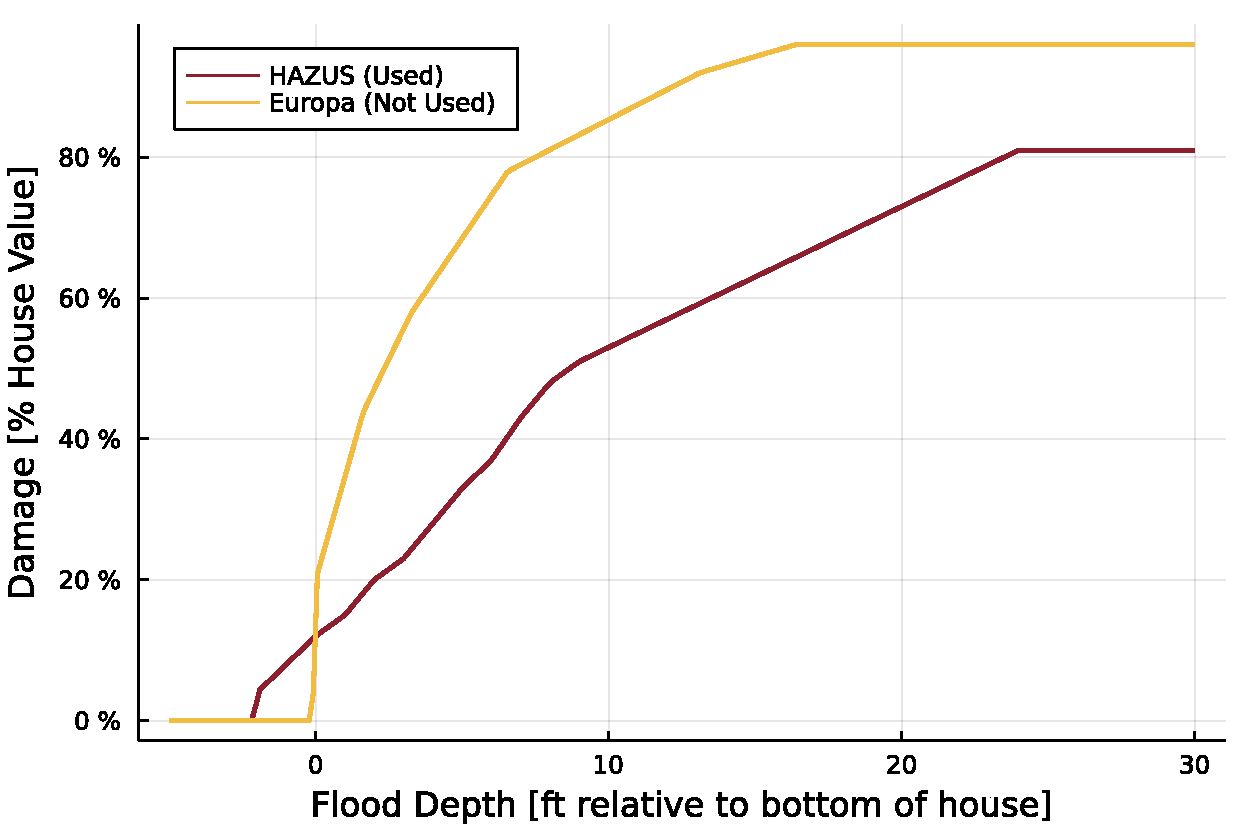
\includegraphics[width=4in]{cost-depth-damage}
    \caption{
        Depth-damage relationship.
        Following \citet{zarekarizi_suboptimal:2020}, we use the Hazard U.S. (HAZUS) depth-damage curves provided by FEMA.
        Since results are sensitive to choice of depth-damage equation, we illustrate (for comparison only) the ``Europa'' depth-damage relationship developed by the Joint Research Center (JRC) of the European Commission's science and knowledge service \citep{huizinga_depthdamage:2016}.
    }\label{fig:cost-depth-damage}
\end{figure}

\begin{figure}
    \centering
    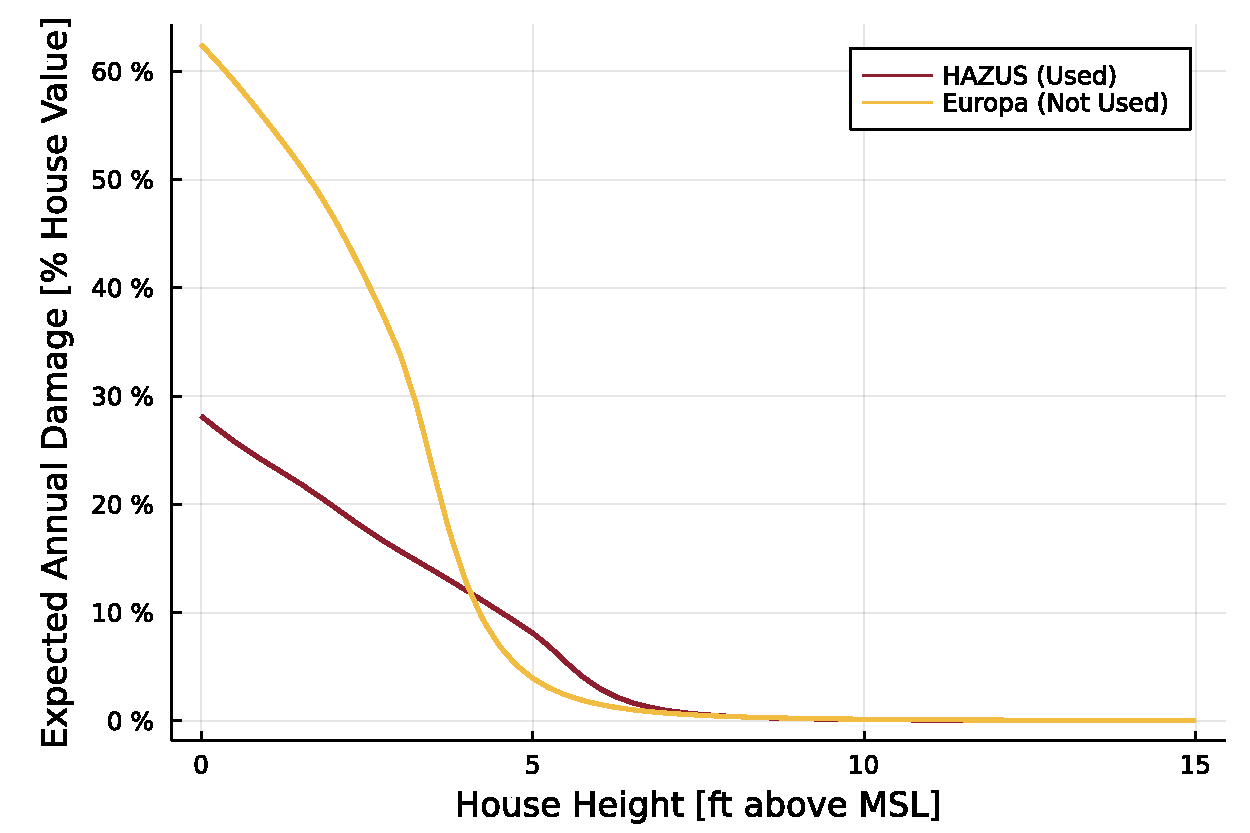
\includegraphics[width=4in]{cost-expected-damage-emulator}
    \caption{
        As discussed in \cref{sec:ead}, we model expected annual damages (eq.~\ref{eq:ead}) as a function of the house's elevation relative to \gls{msl}.
        Damages ($y$ axis) are shown as a percentage of house value.
    }\label{fig:cost-expected-damage-emulator}
\end{figure}

\begin{figure}
    \centering
    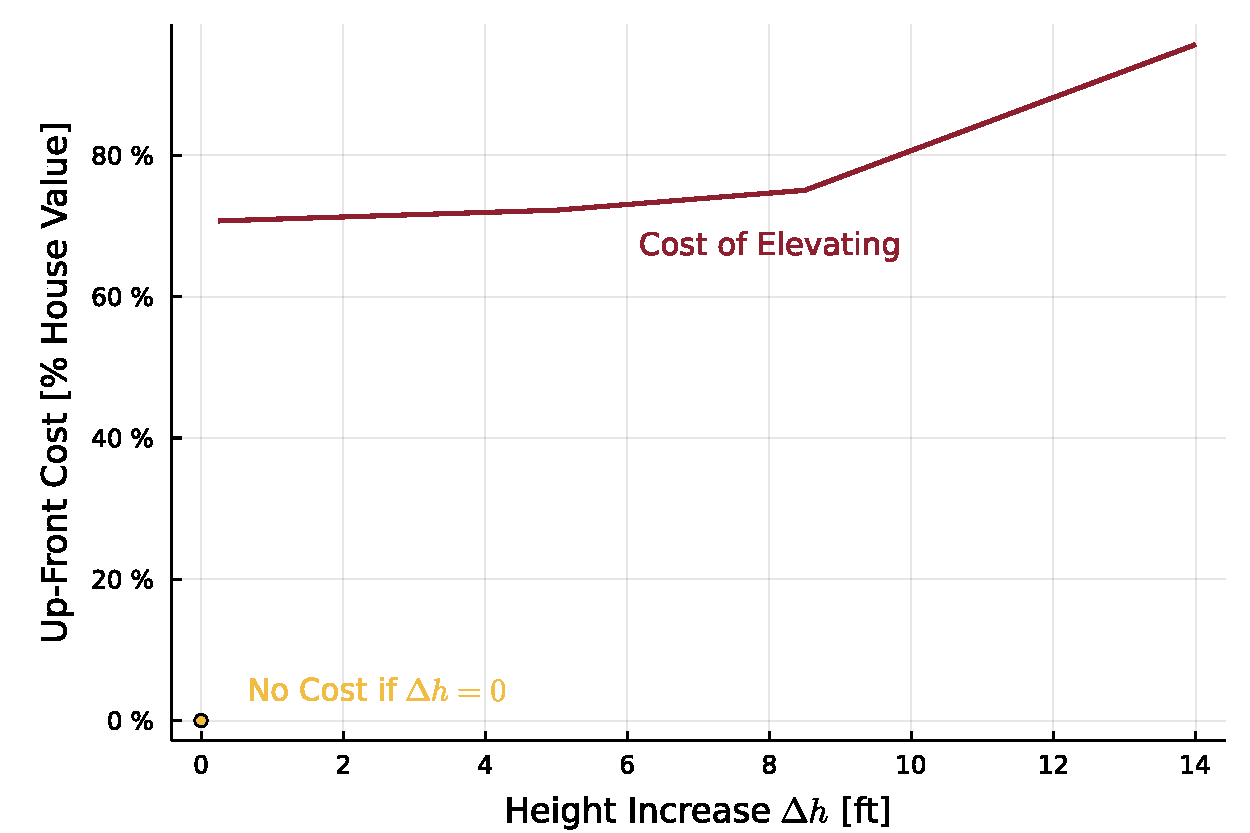
\includegraphics[width=4in]{cost-up-front}
    \caption{
        Following \citet{zarekarizi_suboptimal:2020}, we model the cost of elevating a single-family house by interpolating estimates from the Coastal Louisiana Risk Assessment Model \citep{johnson_clara:2013}.
        According to this model, the unit cost of elevating a house by 3-7, 7-10, and 10-14 feet is \usd{82.50}, \usd{86.25}, and \usd{103.75} per square foot, respectively, with a \usd{20745} initial cost.
        Values are sensitive to house floor area and structural value; see \cref{tab:uncertainties}.
    }\label{fig:cost-up-front}
\end{figure}

\begin{figure}
    \centering
    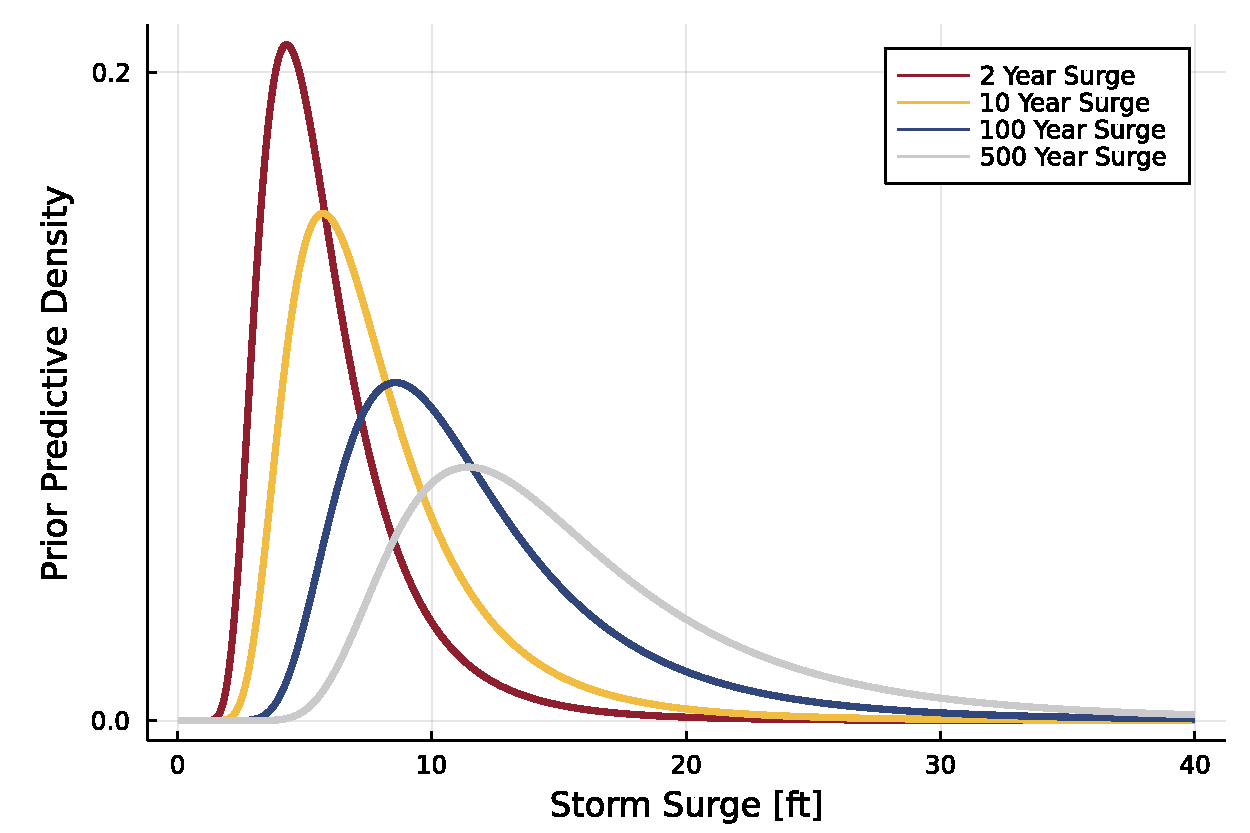
\includegraphics[width=4in]{surge-gev-priors}
    \caption{
        Prior distributions for annual maximum storm surge.
        Rather than apply a prior over model parameters directly, we apply a weakly informative prior over quantiles of the resulting distribution (that is, over a function of the model parameters) following \citet{coles_evd:1996}.
        See \cref{sec:storm-surge} for details.
        For the 2, 10, 100, and 500 year events we apply Normal distributions, truncated at zero, with means \SIlist{4;6;10;15}{ft} and standard deviations \SIlist{1.5;1.75;2.25;2.75}{ft}, respectively.
    }\label{fig:surge-gev-priors}
\end{figure}

\begin{figure}
    \centering
    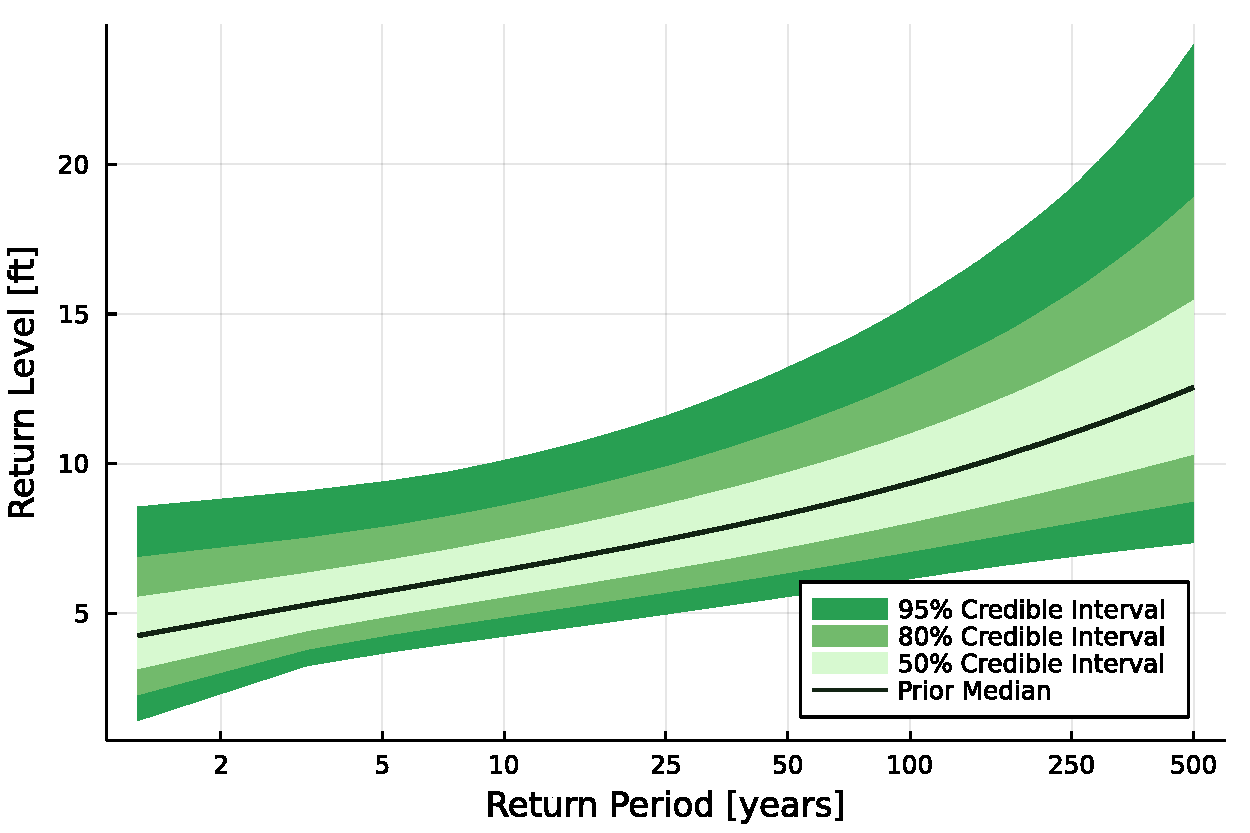
\includegraphics[width=\textwidth]{surge-prior-return}
    \caption{
        Surge prior
    }\label{fig:surge-prior-return}
\end{figure}

\begin{figure}
    \centering
    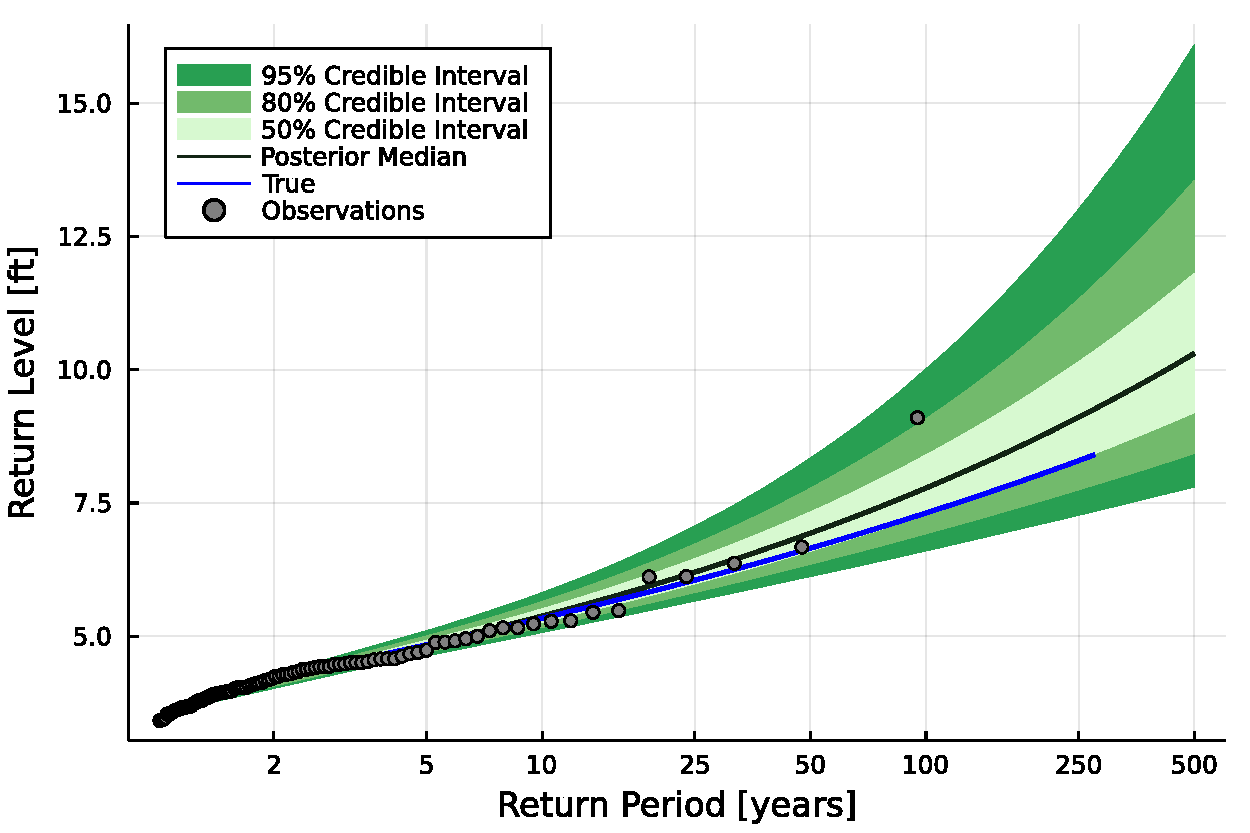
\includegraphics[width=\textwidth]{surge-synthetic-data-experiment}
    \caption{
        Synthetic data experiment as a positive control test for the \gls{gev} model of storm surge.
        A synthetic record was sampled from a \gls{gev} distribution with location, scale, and shape parameters of 4, 0.5, and 0.15, respectively (dots).
        These samples were used to fit the Bayesian \gls{gev} model described in \cref{sec:storm-surge}; the gray shading indicates the 50, 80, and 95\% posterior confidence intervals.
        The blue line shows the true quantiles of the (known) \gls{gev} distribution.
        By random chance the sample maximum has a true return period of $\gg 250$ years, which increases the upper confidence interval of the estimated return probabilities, but the true value is nevertheless within the 50\% posterior confidence interval.
        This experiment yields similar results for alternative values of the known \gls{gev} distribution, and for different random seeds (not shown).
    }\label{fig:surge-synthetic-data-experiment}
\end{figure}

\begin{figure}
    \centering
    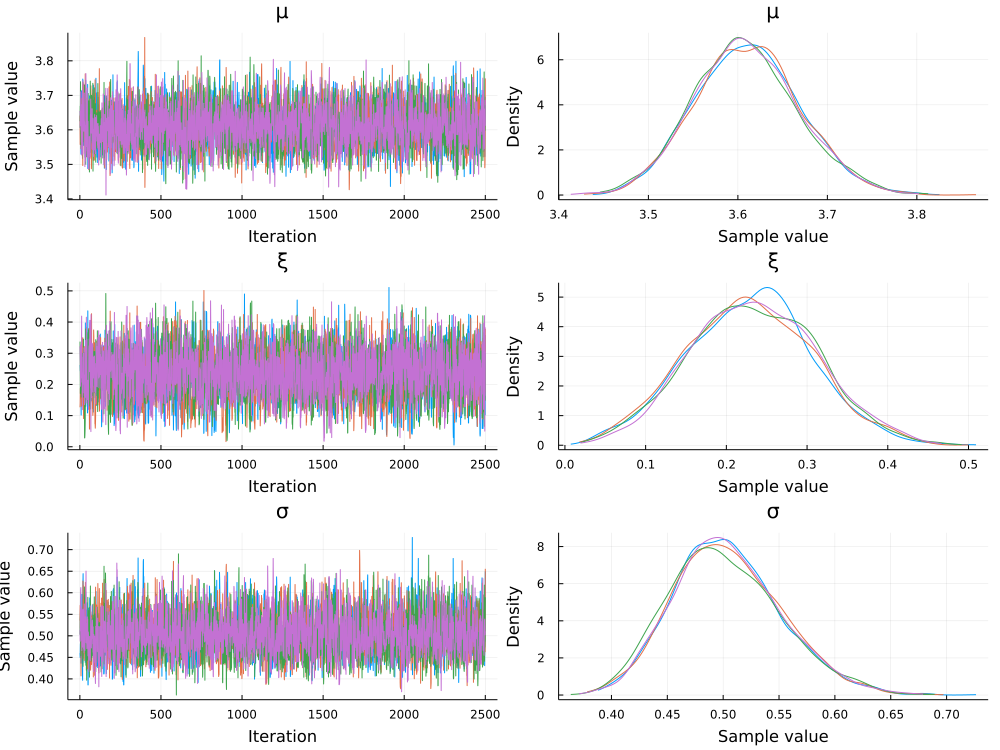
\includegraphics[width=\textwidth]{surge-posterior-chains}
    \caption{
        \Gls{mcmc} plots for posterior draws from the storm surge model.
        We draw \num{10000} samples by running four chains of \num{3500} iterations each and discarding the first \num{1000}.
        The mixing of the chains is consistent with, though does not guarantee, convergence.
    }\label{fig:surge-posterior-chains}
\end{figure}

\begin{figure}
    \centering
    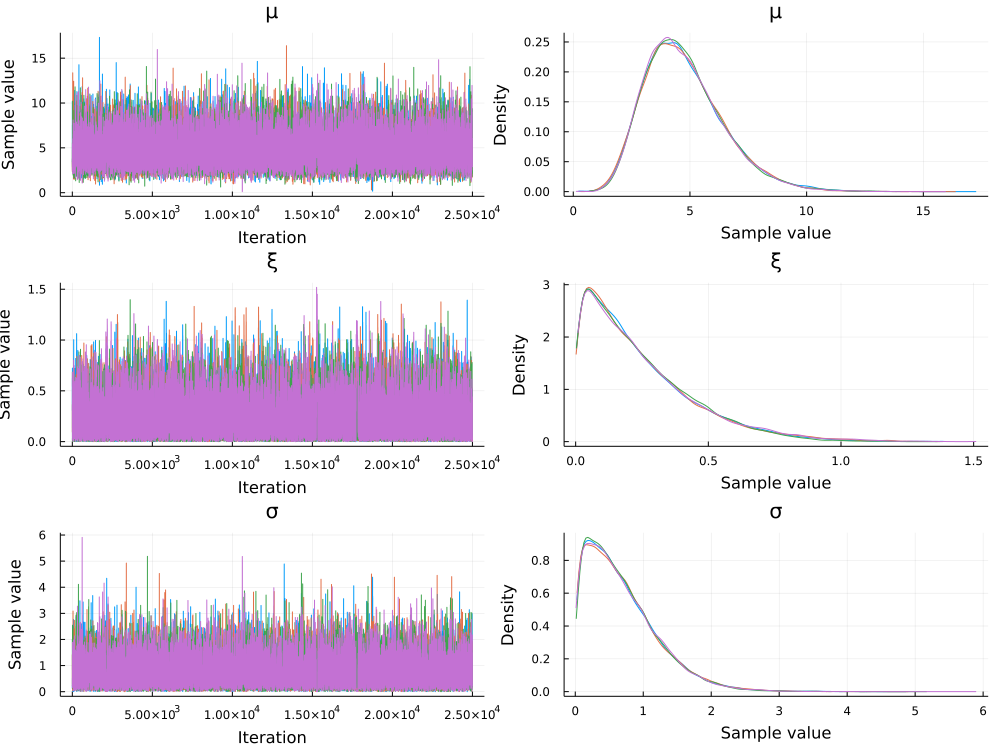
\includegraphics[width=\textwidth]{surge-prior-chains}
    \caption{
        As \cref{fig:surge-posterior-chains} but for draws from the prior distribution.
    }\label{fig:surge-prior-chains}
\end{figure}

\begin{figure}
    \centering
    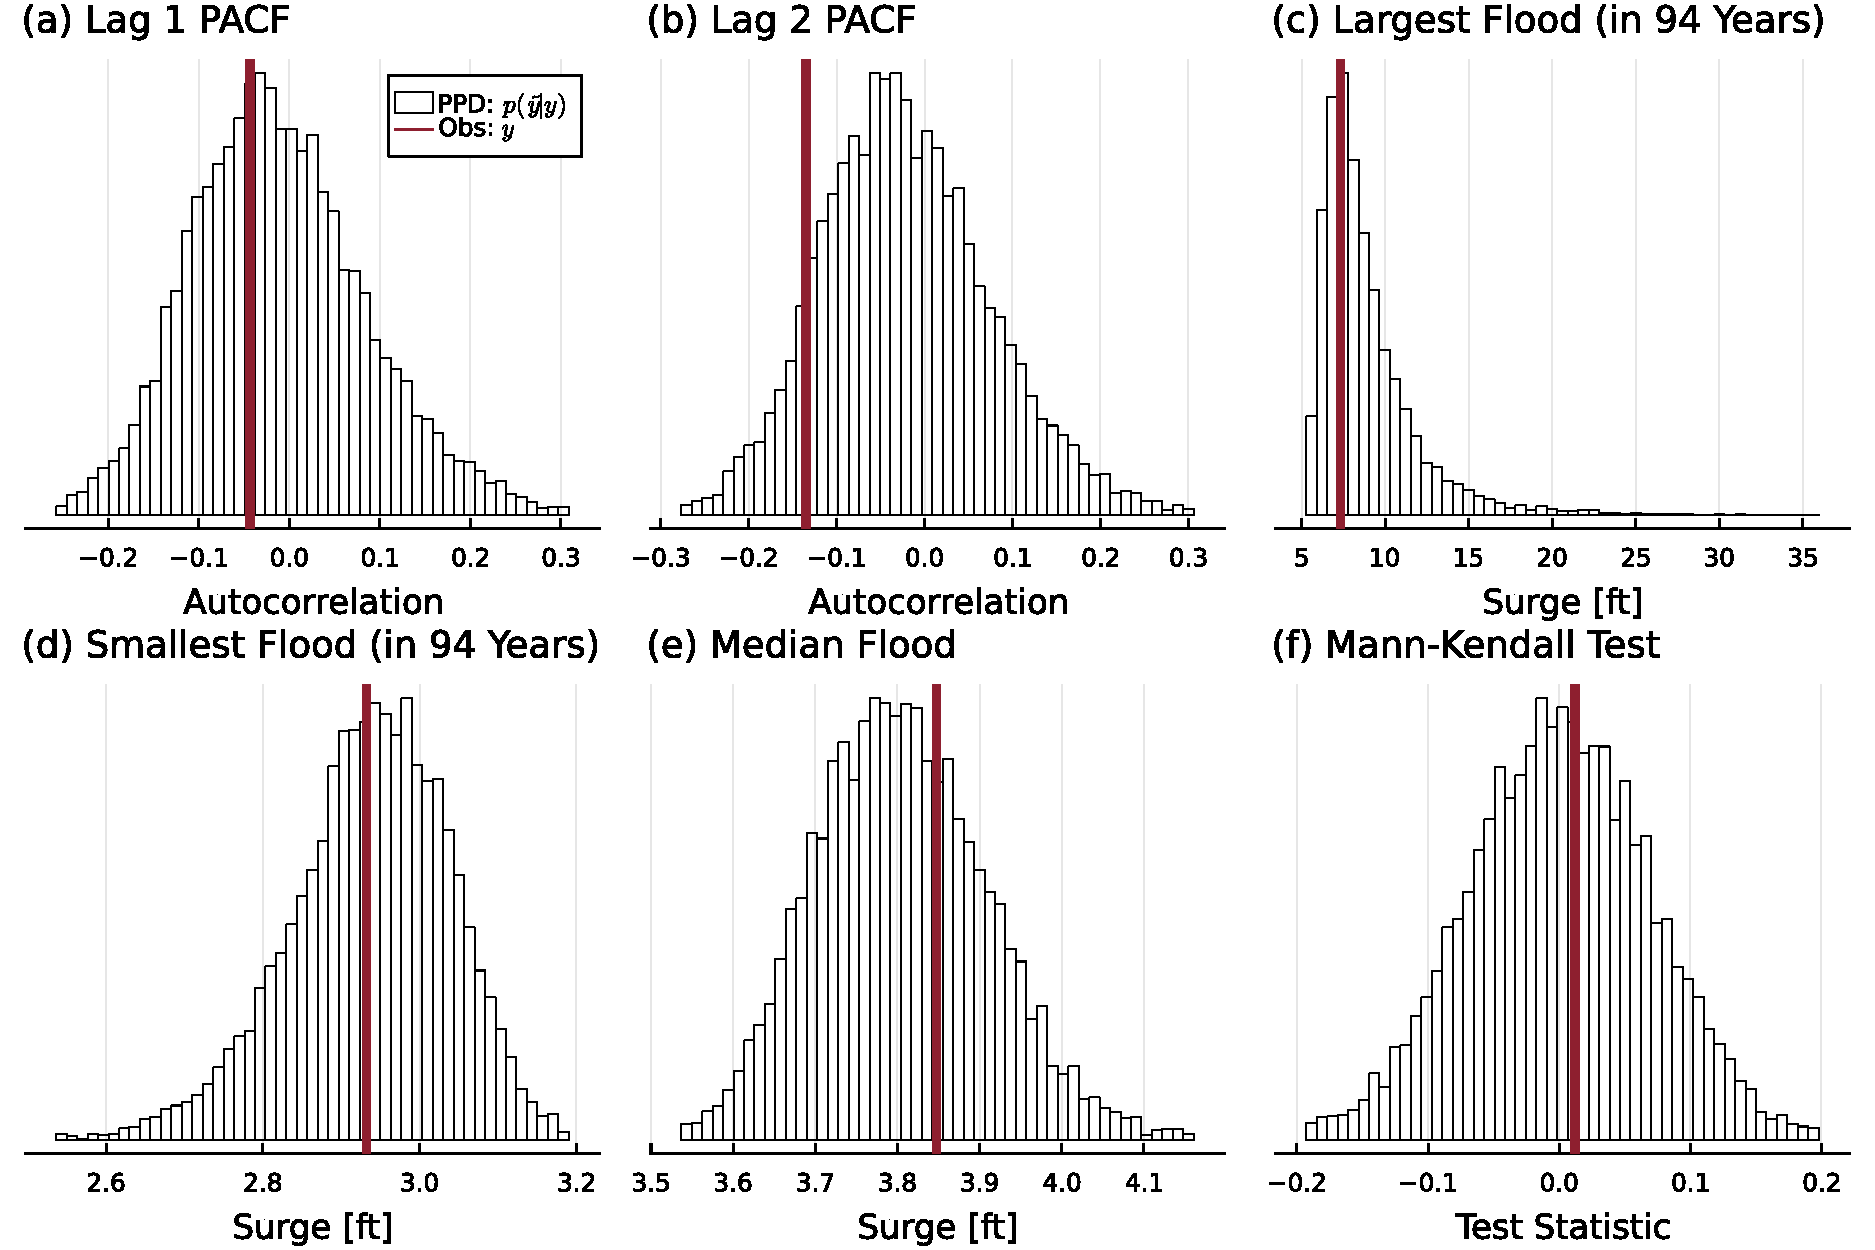
\includegraphics[width=\textwidth]{surge-test-statistics}
    \caption{
        Posterior predictive checks for the stationary \gls{gev} storm surge model (\cref{sec:storm-surge}).
        Each panel shows a different test statistic: partial autocorrelation at lags 1 and 2; sample maximum; sample minimum; sample median; and Mann-Kendall trend test statistic.
        The histograms show the distribution of each test statistic from the posterior predictive distribution.
        Orange lines show the test statistic's value in the observed data.
        Observed values near the mode of the posterior predictive distribution are consistent with, but do not guarantee, a good fit.
        For further discussion of posterior predictive checks, see Chapter 6 of \citet{Gelman:2014tc}.
    }\label{fig:surge-test-statistics}
\end{figure}

\begin{figure}
    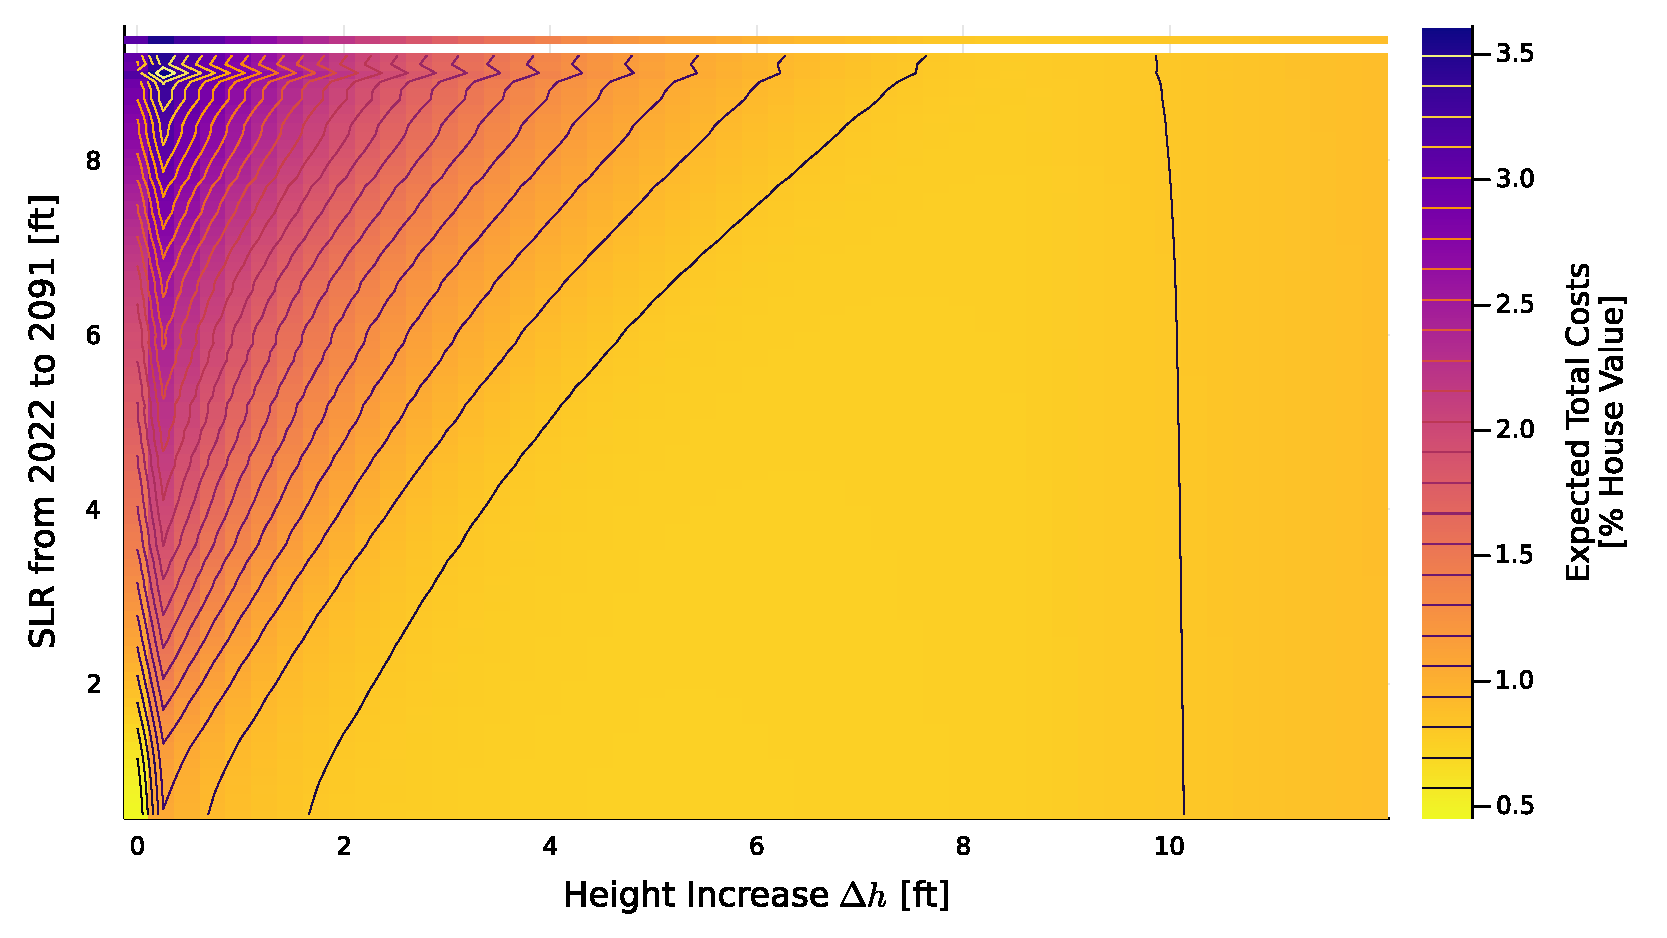
\includegraphics[width=\textwidth]{scenario-map-height-slr}
    \caption{
        Expected total lifetime cost (damages plus up-front cost) as a function of \gls{slr} over the house lifetime and height increase $\Delta h$.
        Initial house elevation is fixed to \SI{1}{ft} below the \gls{bfe}.
    }\label{fig:scenario-map-height-slr}
\end{figure}

\section{Supplemental tables}

\begin{table}[h]
    \centering
    \caption{
        Diagnostic statistics for the \gls{mcmc} sampling for the storm surge posterior draws.
        Statistics include the mean and standard deviation of each parameter, the naive standard error and Monte Carlo standard error (which measure uncertainty in the mean), the effective sample size, $\hat{R}$ diagnostic, and effective samples per second, which describes sampling speed.
        In general, a $\hat{R}$ value close to one is consistent with, though does not guarantee, convergence.
    }\label{tab:surge-posterior-mcmc-diagnostics}
    \begin{tabular}{cccccccc}
\toprule
$\textrm{Parameter}$ & $\textrm{Mean}$ & $\textrm{Stdev.}$ & $\textrm{Naive SE}$ & $\textrm{MCSE}$ & $\textrm{ESS}$ & $\hat{R}$ & $ess_{per\_sec}$\\
\midrule
$\mu$ & $3.610$ & $0.058$ & $0.001$ & $0.001$ & $4819.426$ & $1.000$ & $467.044$\\
$\sigma$ & $0.504$ & $0.049$ & $0.000$ & $0.001$ & $4508.859$ & $1.000$ & $436.947$\\
$\xi$ & $0.231$ & $0.078$ & $0.001$ & $0.001$ & $4729.255$ & $1.001$ & $458.306$\\
\bottomrule
\end{tabular}

\end{table}

\begin{table}[h]
    \centering
    \caption{As \cref{tab:surge-posterior-mcmc-diagnostics} but for draws from the prior distribution.}\label{tab:surge-prior-mcmc-diagnostics}
    \begin{tabular}{ccccccc}
\toprule
$\textrm{Parameter}$ & $\textrm{Mean}$ & $\textrm{Stdev.}$ & $\textrm{Naive SE}$ & $\textrm{MCSE}$ & $\textrm{ESS}$ & $\hat{R}$\\
\midrule
$\mu$ & $4.774$ & $1.702$ & $0.005$ & $0.011$ & $26657.405$ & $1.000$\\
$\xi$ & $0.246$ & $0.215$ & $0.001$ & $0.002$ & $11238.145$ & $1.000$\\
$\sigma$ & $0.682$ & $0.531$ & $0.002$ & $0.004$ & $24720.263$ & $1.000$\\
\bottomrule
\end{tabular}

\end{table}

\end{document}
